\باب{تابع وقت نظریہ اضطراب}\شناخت{باب_تابع_وقت_نظریہ_اضطراب}
%this chapter's  typing is complete 

اب تک ہم جو کچھ کر چکے ہیں اس کو  کوانٹم سکونیات کہا جا سکتا ہے جس میں مخفی توانائی تفاعل غیر تابع وقت ہے \عددی{V(r, t)=V(r)}۔ ایسی صورت میں تابع وقت شروڈنگر مساوات
\begin{align*}
	H\psi=i\hslash\frac{\partial\psi}{\partial t}
\end{align*}
کو علیحدگی متگیرات سے حل کیا جا سکتا ہے 
\begin{align*}
	\psi(r, t) = \psi(r)e^{-iEt/\hslash}
\end{align*}
جہاں \عددی{\psi(r)} غیر تابع شروڈنگر مساوات	
\begin{align*}
	H\psi=E\psi
\end{align*}
کو متمعن کرتا ہے۔ چونکہ علیحدگی حلوں میں تابعیت وقت کو قوت نمائی جز ضربی \عددی{e^{iEt/\hslash}} ظاہر کرتا ہے جو کسی بھی طبعی مقدار کے حصول میں منسوخ ہوتا ہے \عددی{\abs{\psi}^2} لحاظہ تمام احتمالات اور توقعاتی قیمتیں وقت کے لحاظ سے مستقل ہوں گی۔ ان ساکن حالات کے خطی جوڑ تیار کر کے ہم ایساے تفاعلات موج تیار کرسکتے ہیں جن کی تابعیت وقت زیادہ دلچسپ ہو تاہم اب بھی توانائی اور ان کے متعلقہ احتمالات مستقل ہوں گے۔

توانائی کی ایک سطح سے دوسری سطح میں الیکٹران کے انتقال جنہیں بعض اوقات کوانٹم چھلانگ کہتے ہیں کی خاطر ضروری ہے کہ ہم تابع وقت مخفیہ متعارف کریں کوانٹم حرکیات۔ کوانٹم حرکیات میں ایسے بہت کم مسائل پائے جاتے ہیں جن کا حل بلکل ٹھیک ٹھیک معلوم کیا جا سکتا ہے ہاں اگر ہیملٹنی میں غیر تابع وقت حصہ لحاظ سے تابع وقت حصہ بہت چھوٹا ہو تب ہم اسے اضطراب تصور کر سکتے ہیں۔ اس باب میں میںتابع وقت نظریہ اضطراب تیرا کرتا ہوں اور اس کا اطلاق جوہر سے اشعاعی اخراج اور انجزاب پر کرتا ہوں جو اس کی اہم ترین استعمال ہے۔
\حصہ{دو سطحی نظام}
شروعات کنے کی غرض سے فرض کریں غیر مضطرب نظام کے صرف دو حالات \عددی{\psi_a} اور \عددی{\psi_b} پائے جاتے ہیں۔ یہ غیر مضطرب ہیملٹنی \عددی{H^0} کے امتیازی حالات ہوں گے
\begin{align}
	H^0\psi_a=E_a\psi_a,&&\text{\RL{اور}}&&H^0\psi_b=E_b\psi_b
\end{align}
اور معیاری عمودی ہوں گے
\begin{align}
	\langle\psi_a\mid\psi_b\rangle=\delta_{ab}
\end{align}
کسی بھی حال کو ان کا خطی جوڑ لکھا جا سکتا ہے بلخصوص درج ذیل
\begin{align}
	\psi(0)=c_a\psi_a+c_b\psi_b
\end{align}
اس سے فرق نہیں پڑتا کے تفاعلات \عددی{\psi_a} اور \عددی{\psi_b} موزا وہ فضائی تفاعلات یا چکر کار یا کوئی اور عجیب تفاعل ہوں ہمیں یہاں صرف تابیعت وقت سے غرض ہے لحاظہ میں \عددی{\psi(t)} لکھتا ہوں جس سے میرا مراد وقت \عددی{t} پر نظام کا حال ہے۔ عدم اجطراب کی صورت میں ہر جز اپنی خصوصی قوت نمائی جز ضرن کے ساتھ ارتقا پائے گا 
\begin{align}
	\psi(t)=c_a\psi_ae^{-iE_at/\hslash}+c_b\psi_be^{-iE_bt/\hslash}
\end{align}
ہم کہتے ہیں کہ حال \عددی{\psi_a} میں ذرہ پائے جانے کا احتمال \عددی{\abs{c_a}^2} ہے جس سے ہمارا اصل مطلب یہ ہے کہ پیمائش سے  توانائی کی قیمت \عددی{E_a} حال حاصل ہونے کا احتمال \عددی{\abs{c_a}^2} ہوگا۔ تفاعل \عددی{\psi} کی معمولزنی کے تحت درج ذیل ہوگا
\begin{align}
	\abs{c_a}^2+\abs{c_b}^2=1
\end{align}
\جزوحصہ{مضطرب نظام}
اب فرض کریں ہم تابع وقت اضطراب \عددی{H'(t)} چالو کرتے ہیں۔ چونکہ \عددی{\psi_a} اور \عددی{\psi_b} ایک مکمل سلسلہ  مرتب  کرتے ہیں لحاظہ تفاعل موج \عددی{\psi(t)} کو بھی انکا خطی جوڑ لکھا جا سکتا ہے۔ فرق صرف اتنا ہو گا کہ اب \عددی{c_a} اور \عددی{c_b} وقت \عددی{t} کے تفاعلات ہوں گے
\begin{align}
	\psi(t)=c_a(t)\psi_ae^{-iE_at/\hslash}+c_b(t)\psi_be^{-E_bt/\hslash}
\end{align}
میں وقت نمائی  جز ضربیوں کو \عددی{c_a(t)} یا \عددی{c_b(t)} میں ضم کر سکتا ہوں جیسا کے نعض لوگ کرنا پسند کرتے ہیں لیکن میں چاہتا ہوں کے تابعیت وقت کا وہ حصہ جو عدم اضطراب کے  صورت میں بھی پایا جاتا ہو ہمیں نظر آتا رہے ہمارا پورا کام صرف اتنا ہے کہ ہم وقت کے تفاعالات \عددی{c_a} اور \عددی{c_b} تعین کریں۔ مثال کے طور پر اگر ایک ذرہ آغاز میں حال \عددی{\psi_a(c_a(0)=1, c_b(0)=0)} میں پایا جاتا ہو اور بعد میں کسی وقت \عددی{t_1} پر \عددی{c_a(t_1)=0, c_b(t_1)=1} میں پایا جاتا ہو تب ہم کہیں گے کہ نظام \عددی{\psi_a} سے \عددی{\psi_b} میں منتقل ہوا ہے۔

ہم \عددی{c_a(t)} اور \عددی{c_b(t)} معلوم کرنے کی غرض سے مطالبہ کرتے ہیں کہ \عددی{\psi(t)} تابع وقت شروڈنگر مساوات کو متمعن کرے 
\begin{align}
	H\psi=i\hslash\frac{\partial\psi}{\partial t},&&\text{\RL{جہاں}}H=H^0+H'(t)
\end{align}
\حوالہء{مساوات \num{9.6} اور \num{9.7}} سے درج ذیل حاصل ہوگا
\begin{align*}
	c_a[H^0\psi_a]e^{-iE_at/\hslash}+c_b[H^0\psi_b]e^{-iE_bt/\hslash}+c_a[H'\psi_a]e^{-iE_at/\hslash}+c_b[H'\psi_b]e^{-iE_bt/\hslash} \\
	=i\hslash\left[\dot{c}_a\psi_ae^{-iE_at/\hslash}+\dot{c}_b\psi_be^{-iE_bt/\hslash}+c_a\psi_a\left(-\frac{iE_a}{\hslash}\right)e^{-iE_at/\hslash}+c_b\psi_b\left(-\frac{iE_b}{\hslash}\right)e^{-iE_bt/\hslash}\right]
\end{align*}
\حوالہء{مساوات \num{9.1}} کی بدولت بائیں ہاتھ کے پہلے دو اجزا  دائیں ہتھ کے آکری دو اجزا کے ساتھ کٹ جاتے ہیں لحاظہ درج ذیل رہ جائے گا
\begin{align}
	c_a[H'\psi_a]e^{-iE_at/\hslash}+c_b[H'\psi_b]e^{-iE_bt/\hslash}=i\hslash\left[\dot{c}_a\psi_ae^{-iE_at/\hslash}+\dot{c}_b\psi_be^{-iE_bt/\hslash}\right]
\end{align}
تفاعل \عددی{\psi_a} کے ساتھ اندرونی ضرب لیکر \عددی{\psi_a} اور \عددی{\psi_b} کی عمودیت \حوالہء{مساوات \num{9.2}} بروہِ کار لاتے ہوئے \عددی{\dot{c}_a} کو الگ کرتے ہیں
\begin{align*}
	c_a\langle\psi_a\mid H'\mid\psi_a\rangle e^{-iE_at/\hslash}+c_b\langle\psi_a\mid H'\mid\psi_b\rangle e^{-iE_bt/\hslash}=i\hslash\dot{c}_ae^{-iE_at/\hslash}
\end{align*}
مختصر لکھائی کے غرض سے ہم درج ذیل متعارف کرتے ہیں
\begin{align}
	H'_{ij}\equiv\langle\psi_i\mid H'\mid\psi_j\rangle
\end{align}
دیہان رہے کے \عددی{H'} ہرمیشی ہے لحاظہ \عددی{H'_{ji}=(H'_{ij})^*} ہوگا۔ دونوں اطراف کو \عددی{-(i/\hslash)e^{iE_at/\hslash}} سے ضرب دیکر درج ذیل حاصل ہوگا
\begin{align}
	\dot{c}_a=-\frac{i}{\hslash}\left[c_aH'_{aa}+c_bH'_{ab}e^{-i(E_b-E_a)t/\hslash}\right]
\end{align}
اسی طرح \عددی{\psi_b} کے ساتھ اندرونی ضرب سے \عددی{\dot{c}_b} الگ کیا جا سکتا ہے
\begin{align*}
	c_a\langle\psi_b\mid H'\mid\psi_a\rangle e^{-iE_at/\hslash}+c_b\langle\psi_b\mid H'\mid\psi_b\rangle e^{-iE_bt/\hslash}=i\hslash\dot{c}_be^{-iE_bt/\hslash}
\end{align*}
لحاظہ درج ذیل ہوگا 
\begin{align}
	\dot{c}_b=-\frac{i}{\hslash}\left[c_bH'_{bb}+c_aH'_{ba}e^{-i(E_b-E_a)t/\hslash}\right]
\end{align}
\حوالہء{مساوات \num{9.10} اور \num{9.11}} مل کر \عددی{c_a(t)} اور \عددی{c_b(t)} تعین کرتے ہیں یہ دونوں مل کر دو سطحی نظامکی تابع وقت شروڈنگر مساوات کے مکمل معدل ہیں۔ عمومی طور پر \عددی{H'} کے وتری ارکان قالب صفر ہوں گے عمومی صورت کے لیئے \حوالہء{سوال \num{9.4}} دیکھیں
\begin{align}
	H'_{aa}=H'_{bb}=0
\end{align}
اگر ایسا ہو تب مساوات سادہ روپ اختیار کرتی ہے
\begin{align}
	\dot{c}_a=-\frac{i}{\hslash}H'_{ab}e^{-i\omega_0t}c_b,&&\dot{c}_b=-\frac{i}{\hslash}H'_{ba}e^{i\omega_0t}c_a
\end{align}
جہاں درج ذیل ہوگا
\begin{align}
	\omega_0\equiv\frac{E_b-E_a}{\hslash}
\end{align}
میں \عددی{E_b\geq E_a} لوں گا لحاظہ \عددی{\omega_0\geq0} ہوگا۔


\ابتدا{سوال}
ایک ہائڈروجن جوہر کو تابع وقت برقی میدان \عددی{E=E(t)\ak} میں رکھا جاتا ہے۔ زمینی حال \عددی{n=1} اور چار گنا انحطاطی پہلا ہیجان حالات \عددی{n=2} کے بیچ اضطراب \عددی{H'=eEz} کے چاروں قالبی ارکان \عددی{H'_{ij}} کا حساب لگائیں۔ یہ بھی دیکھائیں کہ پانچوں حالات کے لیئے \عددی{H'_{ii}=0} ہوگا۔ تبصرہ محور \عددی{z} کے لحاظ سے طاق ہونے کو بروہِ کار لاتے ہوئے آپ کو صرف ایک تکمل حل کرنا ہوگا۔ اس روپ کے اضطراب زمیہنی حال سے \عددی{n=2} حالات میں سے صرف ایک تک رسائی دیتا ہے لحاظہ زیادہ بلند ہیجان حالات میں منتقلی کو نظرانداز کرتے ہوئے یہ نظام دو حالات تشکیل  کے طور پر کام کرے گا۔
\انتہا{سوال}
\ابتدا{سوال}
غیر تابع وقت اضطراب کی صورت میں \عددی{c_a(0)=1} اور \عددی{c_b(0)=0} لیتے ہوئے \حوالہء{مساوات \num{9.13}} حل کریں۔ تصدیق کیجیئے گا کہ \عددی{\abs{c_a(t)}^2+\abs{c_b(t)}^2=1} ہے۔ تبصرہ: ظاہری طور پر یہ نظام خالص \عددی{\psi_a} اور کسی \عددی{\psi_b} کے بیچ ارتعاش کرتا ہے۔ کیا یہ میرے اس عمومی دعوے کی نفی نہیں کرتا کے غیر تابع وقت اضطراب کی صورت میں انتقال نہیں ہوگا؟ جی نہیں لیکن اس کی وجہ ذرا نازک ہے یہاں \عددی{\psi_a} اور \عددی{\psi_b} نہ کبھی ہیملٹنی کے امتیازی تفاعلات تھے اور نہ ہیں۔ توانائی کی پیمائش کبھی بھی \عددی{E_a} یا \عددی{E_b} نہیں دیگی۔ تابع وقت نظریہ اضطراب میں عمومی طور پر ہم کسی دورانیہ کے لیئے اضطراب چالو کر کے نطام پر نظر ڈالنے کی خاطر اضطراب ختم کرتے ہیں۔ صرف آغاز اور اختتام میں \عددی{\psi_a} اور \عددی{\psi_b} بلکل ٹھیک ہیملٹنی کے امتیازی حالات ہوں گے اور صرف انہی صورتوں میں ہم نظام میں انتقال کی بات کر سکتے ہیں۔ یوں موجودہ مسئلہ میں فرض کیجیئے گا کہ وقت \عددی{t=0} پر اضطراب چالو کیا جاتا ہے جسے وقت \عددی{t} پر منقتع کیا جاتا ہے۔ اس سے آپ کے حساب پر کوئی فرق نہیں پڑے گا تاہم نتائج کی معقول تشریح ممکن ہوگی۔
\انتہا{سوال}
\ابتدا{سوال}
فرض کریں اضطراب کی شکل و صورت وقت کے لحاظ سے \عددی{\delta} تفاعل ہے
\begin{align*}
	H'=U\delta(t)
\end{align*}
جہاں \عددی{U_{aa}=U_{bb}=0} ہے اور \عددی{U_{ab}=U^*_{ba}\equiv\alpha} لیں۔ اگر \عددی{c_a(-\infty)=1} اور \عددی{c_b(-\infty)=0} ہوں تب \عددی{c_a(t)} اور \عددی{c_b(t)} کیا ہوں گے اور کیا \عددی{\abs{c_a(t)}^2+\abs{c_b(t)}^2=1} ہوگا۔ انتقال ہونے کا احتمال \عددی{t\to\infty} کے لیئے \عددی{P_{a\to b}} کیا ہوگا۔ اشارہ: آپ ڈیلٹا تفاعل کو مستطیلوں کی تسلسل کی تحدیدی حد لے سکتے ہیں۔

جواب: \عددی{P_{a\to b}=\sin^2(\abs{\alpha}/\hslash)	} 
\انتہا{سوال}
\جزوحصہ{تابع وقت نظریہ اضطراب}
اب تک سب کچھ بلکل درست رہا ہے ہم نے اضطراب کی جسامت کے بارے میں کچھ فرض نہیں کیا تاہم کم \عددی{H'} کی صورت میں ہم \حوالہء{مساوات \num{9.13}} کو یکِ بعد دیگرِ تخمین سے حل کرسکتے ہیں۔ فرض کریں ذرہ زیریں حال
\begin{align}
	c_a(0)=1,&&c_b(0)=0
\end{align}
سے آغاز کرتا ہے۔ عند اضطراب کی صورت میں ذرہ ہمیشہ کے لیئے یہیں رہے گا۔

\موٹا{رتبہ صفر:}
\begin{align}
	c^{(0)}_a(t)=1,&&c_b^{(0)}(t)=0
\end{align}
میں تخمین کے رتبہ کو زیر، بالا میں کوسین میں لکھتا ہوں۔

ہم \حوالہء{مساوات \num{9.13}} کے دائیں ہاتھ رتبہ صفر کی قیمتیں پر کر کے رتبہ اوّل تخمین حاصل کرتے ہیں۔

\موٹا{رتبہ اوّل:}
\begin{align}
	\begin{matrix}
		\frac{\dif c_a^{(1)}}{\dif t}=0\Rightarrow c_a^{(1)}(t)=1; \\
		\frac{\dif c_b^{(1)}}{\dif t}=-\frac{i}{\hslash}H'_{ba}e^{i\omega_0t}\Rightarrow c_b^{(1)}=-\frac{i}{\hslash}\int_{0}^{t}H'_{ba}(t')e^{i\omega_0t'}\dif t'
	\end{matrix} 
\end{align}
اب ہم انہیں دائیں ہاتھ پُر کر کے رتبہ دوم تخمین حاصل کرتے ہیں۔

\موٹا{رتبہ دوم:}	
\begin{align}
	\begin{matrix}
		\frac{\dif c_a^{(2)}}{\dif t}=-\frac{i}{\hslash}H'_{ab}e^{-i\omega_0t}\left(-\frac{i}{\hslash}\right)\int_{0}^{t}H'{ba}(t')e^{i\omega_0t'}\dif t'\Rightarrow \\
		c_a^{(2)}(t)=1-\frac{1}{\hslash^2}\int_{0}^{t}H'_{ab}(t')e^{-i\omega_0t'}\left[\int_{0}^{t'}H'_{ba}(t'')e^{i\omega_0t''}\dif t''\right]\dif t'
	\end{matrix}
\end{align}
جہاں \عددی{c_b} تبدیل نہیں ہوا \عددی{(c^{(2)}_b(t)=c^{(1)}_b(t))}۔ دیہان رہے کہ \عددی{c^{(2)}_a(t)} میں صفر رتبی جز بھی پایا جات ہے دو رتبی تصحیح صرف تکملی حصہ ہوگا۔

اصولاً ہم اسی طرح چلتے ہوئے \عددی{n}ویں رتبی تخمین کو \حوالہء{مساوات \num{9.13}} کے دائیں ہاتھ میں پُر کر کے \عددی{n+1}ویں رتبہ کے لیئے حل کر سکتے ہیں۔ رتبہ صفر میں \عددی{H'} کا کوئی جز ضربی نہیں پایا جاتا ہے۔ رتبہ اوّل تصحیح میں \عددی{H'} کا ایک جز ضربی پایا جاتا ہے دو رتبی تصحیح میں \عددی{H'} کے دو جز ضربی پائے جاتے ہیں وغیرہ وغیرہ۔ رتبہ تخمین میں خلل \عددی{\abs{c^{(1)}_a(t)}^2+\abs{c^{(1)}_b(t)}^2\neq1} سے صاف ظاہر ہے بلکل درست عددی سروں کو یقیقناً \حوالہء{مساوات \num{9.5}} پر پورا اترنا ہوگا۔ ہاں \عددی{H'} کی طاقت \عددی{1} تک \عددی{\abs{c^{(1)}_a(t)}^2+\abs{c^{(1)}_b(t)}^2} ایک کے برابر ہے اور رتبہ اوّل تخمین سے صرف اتنی ہی توقع کی جاسکتی ہے زیادہ بلند رتبی تخمین کے لیئے بھی ایسا ہوگا۔

\ابتدا{سوال}
فرض کریں آپ \عددی{H'_{aa}=H'_{bb}=0} نہیں لیتے ہیں۔

(الف) اس صورت میں جب \عددی{c_a(0)=1, c_b(0)=0} ہو رتبہ اوّل نظریہ اضطراب سے \عددی{c_a(t)} اور \عددی{c_b(t)} حاصل کریں۔ دیکھائیں کہ \عددی{H'} کی طاقت ایک تک \عددی{\abs{c^{(1)}_a(t)}^2+\abs{c^{(1)}_b(t)}^2=1}۔

(ب) اس مسئلہ کو بہتر انداز سے نمٹا جاسکتا ہے درج ذیل لیکر
\begin{align}
	\dif_a\equiv e^{\frac{i}{\hslash}\int_{0}^{t}H'_{aa}(t')\dif t'}c_a,&&\dif_b\equiv e^{\frac{i}{\hslash}\int_{0}^{t}H'_{bb}(t')\dif t'}c_b
\end{align}
دیکھائیں کہ درج ذیل ہوگا 
\begin{align}
	\dot{\dif}_a=-\frac{i}{\hslash}e^{i\phi}H'_{ab}e^{-i\omega_0t}\dif_b;&&\dot{\dif}_b=-\frac{i}{\hslash}e^{-i\phi}H'_{ba}e^{i\omega_0t}\dif_a
\end{align}
جہاں درج ذیل ہے
\begin{align}
	\phi(t)\equiv\frac{1}{\hslash}\int_{0}^{t}[H'_{aa}(t')-H'_{bb}(t')]\dif t'
\end{align}
یوں \عددی{H'} کےساتھ اضافی جز ضرب \عددی{e^{i\phi}} منسلک ہونے کے علاوہ \عددی{\dif_a} اور \عددی{\dif_b} کی مساواتیں ساخت کے لحاظ سے \حوالہء{مساوات \num{9.13}} کے متماثل ہیں۔

(ج) رربہ اوّل نظریہ اضطراب سے جز (ب) کی ترکیب استعمال کرتے ہوئے \عددی{c_a(t)} اور \عددی{c_b(t)} حاصل کریں۔ اپنے جواب کا جز (الف) کے ساتھ موازنہ کریں دونوں میں فرق پر تبصرہ کریں۔
\انتہا{سوال}
\ابتدا{سوال}
عمومی صورت \عددی{c_a(0)=a, c_b(0)=b} کے لیئے نظریہ اضطراب سے \حوالہء{مساوات \num{9.13}} کو رتبہ دوم تک حل کریں۔
\انتہا{سوال}
\ابتدا{سوال}
غیر تابع وقت اضطراب \حوالہء{سوال \num{9.2}} کے لیئے \عددی{c_a(t)} اور \عددی{c_b(t)} کو رتبہ دوم تک حاصل کریں۔ اپنے جواب کا بلکل ٹھیک نتیجہ کے ساتھ موازنہ کریں۔
\انتہا{سوال}
%==================
%the above is prob 9.6


\جزوحصہ{سائن نما اضطراب}
فرض کریں اضطراب میں تابعیت وقت سائن نما ہو 
\begin{align}
	H'(r, t) = V(r)\cos(\omega t)
\end{align}
تب درج ذیل ہوگا
\begin{align}
	H'_{ab}=V_{ab}\cos(\omega t)
\end{align}
جہاں \عددی{V_{ab}} درج ذیل ہے
\begin{align}
	V_{ab}\equiv\langle\psi_a\mid V\mid\psi_b\rangle
\end{align}
عملاً تقریباً ہر صورت میں وتری قالبی ارکان صفر ہوتے ہیں لحاظہ پہلے کی طرح یہاں بھی میں یہی فرض کروں گا۔ یہاں سے آگے چلتے ہوئے ہم صرف رتبہ اوّل تک متغیرات تلاش کریں گے لحاظہ زیرِ بالا میں تربہ کی نشاندہی نہیں کی جائے گی۔ رتبہ اوّل تک درج ذیل ہوگا \حوالہء{مساوات \num{9.17}} 
\begin{align}
	c_b(t) &\cong-\frac{i}{\hslash}V_{ba}\int_{0}^{t}\cos(\omega t')e^{i\omega_0 t'}\dif t' = -\frac{iV_{ba}}{2\hslash}\int_{0}^{t}\left[e^{i(\omega_0+\omega)t'}+e^{i(\omega_0-\omega)t'}\right]\dif t' \nonumber \\
	&=-\frac{V_{ba}}{2\hslash}\left[\frac{e^{i(\omega_0+\omega)t}-1}{\omega_0+\omega}+\frac{e^{i(\omega_0-\omega)t}-1}{\omega_0-\omega}\right]
\end{align}
یہی جواب ہے لیکن اس کے ساتھ کام کرنا ذرا دشوار ہوگا۔ انتقالی تعدد \عددی{\omega_0} کے بہت قریب جبری تعدد \عددی{\omega} پر توجہ رکھنے سے چکور کوسین میں دوسرا جزو غالب ہوگا جس سے چیزیں بہت آسان ہوجاتی ہیں۔ ہم درج ذیل فرض کرتے ہیں
\begin{align}
	\omega_0+\omega\gg\abs{\omega_0-\omega}
\end{align}
یہ کوئی بہت بڑی پابندی نہیں ہے چونکہ کسی دوسری تعدد پر انتقلا کا احتمال نہ ہونے کے برابر ہوگا۔ یوں پہلے جزو کو نظرانداز کرتے ہوئے درج ذیل لکھا جا سکتا ہے
\begin{align}
	c_b(t) &\cong-\frac{V_{ba}}{2\hslash}\frac{e^{i(\omega_0-\omega)t/2}}{\omega_0-\omega}\left[e^{i(\omega_0-\omega)t/2}-e^{-i(\omega_0-\omega)t/2}\right]\nonumber \\
	&=-i\frac{V_{ba}}{\hslash}\frac{\sin[(\omega_0-\omega)t/2]}{\omega_0-\omega}e^{i(\omega_0-\omega)t/2}
\end{align}
ایک ذرہ جو حال \عددی{\psi_a} سے آغاز کرے کا لمحہ\عددی{t} پر حال \عددی{\psi_b} میں پائے جانے کا احتمال درج ذیل ہوگا جس کو انتقالی احتمال کہتے ہیں 
\begin{align}
	P_{a\to b}(t)=\abs{c_b(t)}^2\cong\frac{\abs{V_{ab}^2}}{\hslash^2}\frac{\sin^2[(\omega_0-\omega)t/2]}{(\omega_0-\omega)^2}
\end{align}
وقت کے لحاظ سے انتقالی احتمال سائن نما ارتعاش کرتا ہے (شکل \حوالہ{شکل_تابع_وقت_احتمال_سائن_نما_احتمال})۔ یہ \عددی{\abs{V_{ab}}^2/\hslash^2(\omega_0-\omega)^2} کی زیادہ سے زیادہ قیمت تک پہنچ کر جو لازمی طور پر ایک  \عددی{(1)} سے بہت کم ہے ورنہ کم اضطراب کا مفروضہ درست نہیں ہوگا یہ واپسصفر کو گرتا ہے۔ لمحات \عددی{t_n=2n\pi/\abs{\omega_0-\omega}} جہاں \عددی{n=1, 2, 3, \dots} ہیں پر ذرہ لاظماً نچلی حال میں ہوگا اگر آپ منتقلی کا احتمال بڑھانا چاہتے ہیں اضطراب کو لمبے عرصہ کے لیئے چالو نہ کریں۔ بہتر ہوگا کہ آپ وقت \عددی{\pi/\abs{\omega_0-\omega}} پر اضطراب کو روک کر نظام کو بالائی حال میں پانے کی اُمید کریں۔ \حوالہء{سوال \num{9.7}} میں آپ دیکھیں گے کہ دو حالات کے بیچ انتقال نظریہ اضطراب کی پیدا کرادہ  مسنوئی خاصیت  نہیں ہے بلکہ بلکل ٹھیک حال میں بھی ایسا ہوگا تاہم منتقلی کا تعدد کچھ مختلف ہوگا۔

\begin{figure}
\centering
\begin{tikzpicture}[declare function={f(\x)= 1-cos(\x);}]
\begin{axis}[axis lines=middle,xlabel={$t$},ylabel={$P(t)$}, xtick={360,720,1080},
 xticklabels={$\tfrac{2\pi}{\abs{\omega_0-\omega}}$ ,$\tfrac{4\pi}{\abs{\omega_0-\omega}}$, $\tfrac{6\pi}{\abs{\omega_0-\omega}}$}, ytick={2}, yticklabels={$\abs{\tfrac{\abs{V_{ab}}}{\hslash(\omega_0-\omega)}}^2$}, ylabel style={at={(current axis.above origin)},anchor=west},xlabel style={at={(current axis.right of origin)},anchor=north east},enlargelimits]
\addplot [thick,samples=100,domain=0:1260]{f(x)};
\addplot [dashed] coordinates{(0,2)(1260,2)};
\end{axis}
\end{tikzpicture}
\caption{سائن نما اضطراب کے لئے وقت کے لحاظ سے تحویلی احتمال (مساوات \حوالہء{9.28})۔}
\label{شکل_تابع_وقت_احتمال_سائن_نما_احتمال}
\end{figure}


جیسا میں ذکر کر چکا ہوں انتقال کی احتمال اس صورت زیادہ سے زیادہ ہوگا جب جبری تعدد قدرتی تعدد \عددی{\omega_0} کے قریب ہو۔ شکل \حوالہ{شکل_تابع_وقت_احتمال_جبری_تعدد}  میں \عددی{\omega} کے لحاظ سے \عددی{P_{a\to b}} ترسیم کر کے اس حقیقت کو اجاگر کیا گیا ہے۔ چوٹی کی اونچائی \عددی{(\abs{V_{ab}t/2\hbar})^2} جبکہ چوڑائی \عددی{4\pi/t} ہے یوں وقت گزرنے کے ساتھ ساتھ اسکی بلندی بڑھتی ہے اور چوڑائی گھٹتی ہے۔ بظاہر زیادہ سے زیادہ قیمت بغیر کسی حد کے بتدریج بڑھتی ہے تاہم ایک پر پہنچنے سے بہت پہلے اضطراب کا مفروضہ ناکرا ہو جاتا ہے۔ لحاظہ ہم بہت کم \عددی{t} کے لیئے اس نتیجہ پر یقین کر سکتے ہیں۔ \حوالہء{سوال \num{9.7}} میں آپ دیکھیں گے کہ بلکل ٹھیک ٹھیک نتیجہ کبھی بھی ایک سے ایک تجاوز نہیں کرتا ہے۔
\begin{figure}
\centering
\pgfmathsetmacro{\k}{15}
\pgfmathsetmacro{\ka}{\k-2*pi}
\pgfmathsetmacro{\kb}{\k+2*pi}
\begin{tikzpicture}[declare function={f(\x)= (sin(deg(\k-\x)/2)^2)/pow(\k-\x,2);}]
\begin{axis}[clip=false,axis lines=middle,xlabel={$\omega$},ylabel={$P(\omega)$}, xtick={\k,\ka,\kb},
 xticklabels={$\omega_0$,,}, ytick={0.25}, yticklabels={}, ylabel style={at={(current axis.above origin)},anchor= east},xlabel style={at={(current axis.right of origin)},anchor=north},enlargelimits]
\addplot [thick,smooth,domain=0:30,samples=50]{f(x)};
\addplot[] coordinates {(\ka,0)}node[pin=-120:{$(\omega_0-2\pi/t)$}]{};
\addplot[] coordinates {(\kb,0)}node[pin=-60:{$(\omega_0+2\pi/t)$}]{};
\end{axis}
\end{tikzpicture}
\caption{تحویلی احتمال بالمقابل   متحرک  تعدد  (مساوات \حوالہء{9.28})۔}
\label{شکل_تابع_وقت_احتمال_جبری_تعدد}
\end{figure}


\ابتدا{سوال}
پہلا جزو \حوالہء{مساوات \num{9.25}} میں \عددی{\cos(\omega t)} کے \عددی{e^{i\omega t}/2} سے جبکہ دوسرا \عددی{e^{-i\omega t}/2} سے آتا ہے یوں پہلے جزو کو  نظرانداز کرنا باضابطہ طور پر \عددی{H'=(V/2)e^{-i\omega t}} لکھنے کا معادل ہے یعنی ہم درج ذیل کہہ سکتے ہیں
\begin{align}
	H'_{ba}=\frac{V_{ba}}{2}e^{-i\omega t},&&H'_{ab}=\frac{V_{ab}}{2}e^{i\omega t}
\end{align}
ہیملٹنی قالب کو ہرمیشی بنانے کی خاطر مئاخر الذکر کی ضرورت پیش آتی ہے۔ آپ کہہ سکتے ہیں ہم \عددی{c_a(t)} کے لیئے \حوالہء{مساوات \num{9.25}} کی طرح کلیہ میں غالب جزو کو چنتے ہیں۔ اسکو گھومتی موج تخمین کہتے ہیں جناب رابی نے دیکھا کہ حساب کی آغاز میں گھومتی موج تخمین کرتے ہوئے \حوالہء{مساوات \num{9.13}} کو بغیر نظریہ اضطراب اور میدان کی زور کے بارے میں کچھ بھی فرض کیئے بغیر بلکل ٹھیک ٹھیک حل کیا جا سکتا ہے۔

(الف) عمومی ابتدائی معلومات \عددی{c_a(0)=1, c_b(0)=0} کے لیئے گھومتی موج تخمین \حوالہء{مساوات \num{9.29}} لیتے ہوئے \حوالہء{مساوات \num{9.13}} حل کریں۔ اپنے جوابات \عددی{c_a(t)} اور \عددی{c_b(t)} کو رابی تعدد 
\begin{align}
	\omega_r\equiv\frac{1}{2}\sqrt{(\omega-\omega_0)^2+(\abs{V_{ab}}/\hslash)^2}
\end{align}
کی صورت میں لکھیں۔

(ب) انتقالی احتمال \عددی{P_{a\to b}(t)} تعین کر کے دیکھائیں کہ یہ کبھی بھی ایک سے تجاوز نہیں کرتا۔ تصدیق کریں کہ \عددی{\abs{c_a(t)}^2+\abs{c_b(t)}^2=1} ہوگا۔

(ج) دیکھیں کہ کم اضطراب کی صورت میں \عددی{P_{a\to b}(t)} عین نظریہ اضطران کے نتیجہ \حوالہء{مساوات \num{9.28}} کے تحت ہوگا۔ سیاق و سباق کے لحاظ سے یہاں کم سے کیا مراد ہے اور \عددی{V} پر یہ کیا پابندی عاید کرتی ہے۔

(د) نظام پہلی بار اپنی ابتدائی حال میں کتنی دیر میں واپس آئے گا؟
\انتہا{سوال}

%below is sec 9.2 onwards till end of chapter

\حصہ{اشعاعی اخراج اور انجذاب}
\جزوحصہ{برقناطیسی امواج}
ایک برقناطیسی موج جس کو میں رشنی کہوں گا اگرچہ یہ زیریں سرخ، بالائے بصری شعاع، خرد امواج، ایکس رے وغیرہ ہو سکتی ہے۔ جن میں صرف تعدد کا فرق ہوتا ہے۔ عرضی اور باہم قائمہ ارتعاشی برقی اور مقناطیسی میدانوں پر مشتمل ہوگا (شکل \حوالہ{شکل_تابع_وقت_احتمال_برقناطیسی_موج})۔ ایک جوہر گزرتی ہوئی بصری موج کی موجودگی میں بنیادی طور پر صرف برقی جز کو ردعمل دیتا ہے۔ اگر طولِ موج جوہر کی جسامت کے لحاظ سے لمبی ہو تب ہم میدان کی فضائی تغیر کو نظرانداز کرسکتے ہیں۔ تب جوہر سائن نما ارتعاشی برقی میدان
\begin{align}
	E = E_0\cos(\omega t)\,\ak
\end{align}
کے زیرِ اثر ہوگا۔ فل حال میں فرض کرتا ہوں کہ روشنی یک رنگی اور \عددی{z} رخ ترتیب شدہ ہے۔ اضطرابی ہیملٹنی درج ذیل ہوگا جہاں \عددی{q} الیکٹران کا بار ہے ۔
\begin{align}
	H^\prime =-qE_0z\cos(\omega t)
\end{align}	

\begin{figure}
\centering
\begin{tikzpicture}[x={(-0.5cm,-0.5cm)},y={(1cm,0cm)},z={(0cm,1cm)},declare function={f(\x)=2*sin(\x);}]
\draw[-stealth] (0,0,0) -- (2,0,0) node[left]{$x$};
\draw[-stealth] (0,0,0) -- (0,8,0) node[above]{$y$};
\draw[-stealth] (0,0,0) -- (0,0,2) node[left]{$z$};
%first 180 degrees
\pgfmathsetmacro{\t}{0}
\draw[thick] plot[domain=\t+0:\t+180,smooth]({f(\x)},{0.5 + \x/180},{0}); 
\foreach \x in {30,60,...,150}{\draw[-latex] ({0},{0.5+\x/180},{0}) --++ ({f(\x)},{0},{0});}
\draw[thick] plot[domain=\t+0:\t+180,smooth]({0},{0.5 + \x/180},{f(\x)});
\foreach \x in {30,60,...,150}{\draw[-latex] ({0},{0.5+\x/180},{0}) --++ ({0},{0},{f(\x)});}
%\draw[thick] plot[domain=180+0:180+180,smooth]({f(\x)},{0.5 + \x/180},{0}); 
% second 180 degrees
\pgfmathsetmacro{\t}{180}
\draw[thick] plot[domain=\t+0:\t+180,smooth]({f(\x)},{0.5 + \x/180},{0}); 
\foreach \x in {210,240,...,330}{\draw[-latex] ({0},{0.5+\x/180},{0}) --++ ({f(\x)},{0},{0});}
\pgfmathsetmacro{\t}{540}
\draw[thick] plot[domain=\t+0:\t+180,smooth]({f(\x)},{0.5 + \x/180},{0}); 
\foreach \x in {570,600,...,690}{\draw[-latex] ({0},{0.5+\x/180},{0}) --++ ({f(\x)},{0},{0});}
\pgfmathsetmacro{\t}{900}
\draw[thick] plot[domain=\t+0:\t+110,smooth]({f(\x)},{0.5 + \x/180},{0}); 
\foreach \x in {930,960,...,990}{\draw[-latex] ({0},{0.5+\x/180},{0}) --++ ({f(\x)},{0},{0});}
%now cutting the magnetic lines
\pgfmathsetmacro{\ct}{360}
\fill[fill=white] plot[domain=\ct+0:\ct+180,smooth]({0},{0.5 + \x/180},{f(\x)}) --cycle;
\draw[thick] plot[domain=\ct+0:\ct+180,smooth]({0},{0.5 + \x/180},{f(\x)});
\foreach \x in {390,410,...,530}{\draw[-latex] ({0},{0.5+\x/180},{0}) --++ ({0},{0},{f(\x)});}
\pgfmathsetmacro{\ct}{720}
\fill[fill=white] plot[domain=\ct+0:\ct+180,smooth]({0},{0.5 + \x/180},{f(\x)}) --cycle;
\draw[thick] plot[domain=\ct+0:\ct+180,smooth]({0},{0.5 + \x/180},{f(\x)});
\foreach \x in {730,760,...,870}{\draw[-latex] ({0},{0.5+\x/180},{0}) --++ ({0},{0},{f(\x)});}
%drawing to be cut portion of electric field
\pgfmathsetmacro{\t}{180}
\draw[thick] plot[domain=\t+0:\t+180,smooth]({0},{0.5 + \x/180},{f(\x)});
\foreach \x in {210,240,...,330}{\draw[-latex] ({0},{0.5+\x/180},{0}) --++ ({0},{0},{f(\x)});}
\pgfmathsetmacro{\t}{540}
\draw[thick] plot[domain=\t+0:\t+180,smooth]({0},{0.5 + \x/180},{f(\x)});
\foreach \x in {570,600,...,690}{\draw[-latex] ({0},{0.5+\x/180},{0}) --++ ({0},{0},{f(\x)});}
\pgfmathsetmacro{\t}{900}
\draw[thick] plot[domain=\t+0:\t+110,smooth]({0},{0.5 + \x/180},{f(\x)});
\foreach \x in {930,960,...,1010}{\draw[-latex] ({0},{0.5+\x/180},{0}) --++ ({0},{0},{f(\x)});}
%cutting electric field
\pgfmathsetmacro{\t}{360}
\fill[fill=white] plot[domain=\t+0:\t+180,smooth]({f(\x)},{0.5 + \x/180},{0}) --cycle;
\draw[thick] plot[domain=\t+0:\t+180,smooth]({f(\x)},{0.5 + \x/180},{0}); 
\foreach \x in {390,410,...,510}{\draw[-latex] ({0},{0.5+\x/180},{0}) --++ ({f(\x)},{0},{0});}
\pgfmathsetmacro{\t}{720}
\fill[fill=white] plot[domain=\t+0:\t+180,smooth]({f(\x)},{0.5 + \x/180},{0}) --cycle;
\draw[thick] plot[domain=\t+0:\t+180,smooth]({f(\x)},{0.5 + \x/180},{0}); 
\foreach \x in {750,780,...,870}{\draw[-latex] ({0},{0.5+\x/180},{0}) --++ ({f(\x)},{0},{0});}
\draw[-latex] (0.5,7,0) --++ (0,0.75,0) node[below,pos=0.5]{\RL{حرکت کا رخ}};
\draw[] ({f(90)}, {0.5+90/180}, {0}) node[pin=-130:{\RL{مقناطیسی میدان}}]{};
\draw[] ({0},{0.5+90/180},{f(90)}) node[pin=45:{\RL{برقی  میدان}}]{};
\end{tikzpicture}
\caption{برقناطیسی موج۔}
\label{شکل_تابع_وقت_احتمال_برقناطیسی_موج}
\end{figure}

ظاہر ہے درج ذیل ہوگا
\begin{align}
	H^{\prime}_{ba} =-pE_0 \cos(\omega t). \text{where} p \equiv q\langle \phi_b \abs{z}\phi_a\rangle
\end{align}
عمومی طور پر \(\psi\) متغیر \عددی{z} کا جفت یا طاق تفاعل ہوگا یہ ہماری اُس مفروضہ کا سبب ہے جس کے تحت ہم کہتے ہیں کہ \(H^\prime\) کے وتری قالبی ارکان صفر ہوں گے۔ یوں روشنی اور مادہ کا باہم عمل ٹھیک اُسی قسم کے ارتعاشی اضطراب کہ تحت ہوگا جن پر ہم نے حصہ 9.3.1 میں غور کیا۔ یہاں درج ذیل ہوگا۔  
\begin{align}
	V_{ba} = -pE_0
\end{align}
\جزوحصہ{انجزاب، تحرق شدہ اخراج اور خود با خود اخراج}
ایک جوہر جو ابتدائی طور پر زیری حال \(\phi_a\) میں پایا جاتا ہو پر تقطیب شدہ یک رنگی روشنی کی شعاع ڈالی جاتی ہے۔ بالائی حال \(\psi_b\) میں انتقال کا احتمال مساوات \num{9.28} دیتی ہے جو مساوات \num{9.34} کی روشنی میں درج ذیل روپ اختیار کرتی ہے۔
\begin{align}
	P_{a\rightarrow b} (t) = (\frac{\abs{p}E_0}{\hbar})^2 \frac{\sin^2[(\omega_0 - \omega)t/2]}{(\omega_0 - \omega)^2}
\end{align}
%
\begin{figure}
\centering
\begin{subfigure}{0.3\textwidth}
\centering
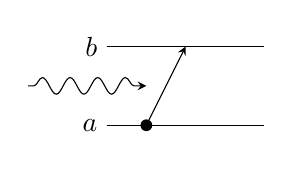
\begin{tikzpicture}
\draw[] (0,0.5) node[left]{$b$} --++ (2,0);
\draw[] (0,-0.5) node[left]{$a$} --++ (2,0);
\draw[-stealth] (0.5,-0.5) node[fill=black,circle,inner sep=1.5pt]{} -- (1,0.5);
\draw[-stealth,decorate,decoration={snake,amplitude=3pt,pre length=2pt,post length=3pt}] (-1,0) --++ (1.5,0);
\end{tikzpicture}
\caption{جذب}
\end{subfigure}\hfill
\begin{subfigure}{0.3\textwidth}
\centering
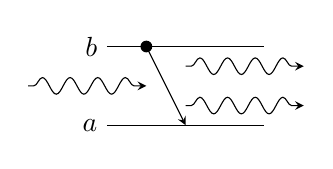
\begin{tikzpicture}
\draw[] (0,0.5) node[left]{$b$} --++ (2,0);
\draw[] (0,-0.5) node[left]{$a$} --++ (2,0);
\draw[-stealth] (0.5,0.5) node[fill=black,circle,inner sep=1.5pt]{} -- (1,-0.5);
\draw[-stealth,decorate,decoration={snake,amplitude=3pt,pre length=2pt,post length=3pt}] (-1,0) --++ (1.5,0);
\draw[-stealth,decorate,decoration={snake,amplitude=3pt,pre length=2pt,post length=3pt}] (1,0.25) --++ (1.5,0);
\draw[-stealth,decorate,decoration={snake,amplitude=3pt,pre length=2pt,post length=3pt}] (1,-0.25) --++ (1.5,0);
\end{tikzpicture}
\caption{تحرک زدہ   اخراج}
\end{subfigure}\hfill
\begin{subfigure}{0.3\textwidth}
\centering
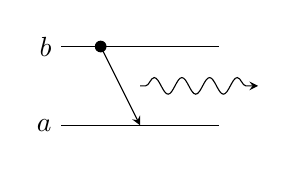
\begin{tikzpicture}
\draw[] (0,0.5) node[left]{$b$} --++ (2,0);
\draw[] (0,-0.5) node[left]{$a$} --++ (2,0);
\draw[-stealth] (0.5,0.5) node[fill=black,circle,inner sep=1.5pt]{} -- (1,-0.5);
\draw[-stealth,decorate,decoration={snake,amplitude=3pt,pre length=2pt,post length=3pt}] (1,0) --++ (1.5,0);
\end{tikzpicture}
\caption{خود بخود  اخراج}
\end{subfigure}
\caption{روشنی  کا جوہر کے ساتھ تین قسم کے باہم عمل پائے جاتے ہیں۔ }
\label{شکل_تابع_وقت_احتمال_روشنی_باہم_عمل}
\end{figure}


اس عمل میں برقناطیسی میدان سے جوہر \(E_b - E_a = \hbar\omega_0\) توانائی جزب کرتا ہے۔ ہم کہتے ہیں اس میں ایک فوٹان جزب کیا (شکل \حوالہ{شکل_تابع_وقت_احتمال_روشنی_باہم_عمل}-ا)۔  جیسا میں ذکر کر چکا ہوں لفظ فوٹان در حقیقت کوانٹم برقی حرقیات برقناطیسی میدان کی کوانٹم نظریہ سے تعلق رکھتا ہے جبکہ ہم میدان کو کلاسیکی نقطہ نظر سے دیکھ رہے ہیں۔ یہ زبان اُس وقت تک استعمال کرنا مناسب ہے جب تک آپ اس سے زیادہ گہرا مطلب نہ لیں۔

یقیناً میں بالائی حال \((c_a(0)=0, c_b(0)=1)\) سے آغاز کرتے ہوئے پورا عمل دوبارہ کرسکتا ہوں۔ آپ سے گزارش ہے کہ ایسا کریں نتائج بلکل وہی ہوں گے البتہ اس بار \(P_{b\rightarrow a} = \abs{C_a(t)}^2\) حاصل ہوگا جو نیطے رخ زیریں لیول میں منتقل کا احتمال ہوگا۔
\begin{align}
	P_{b\rightarrow a} (t) = (\frac{\abs{p}E_0}{\hbar})^2 \frac{\sin^2[(\omega_0 - \omega)t/2]}{(\omega_0 - \omega)^2}
\end{align}
چونکہ ہم \(a\leftrightarrow b\) کو آپس میں بدل رہے ہیں جو \(\omega_0\) کی جگہ \(-\omega_0\) ڈالتا ہے لحاظہ لاظماً یہی نتیجہ حاصل ہوتا مساوات \num{9.25} پر اب پہنچ کر ہم پہلا جز چنتے ہیں جس کے نصب نما میں \(-\omega_0 + \omega\) پایا جاتا ہے باقی حصاب پہلے کی طرح ہے لیکن اگر آپ ایک بار رک کر سوچیں تو یہ نتیجہ حیرت انگیز ہے۔ بالائی حال میں پائے جانے والے ذرہ پر روشنی کی شعاع ڈالنے سے ذرہ زیریں حال میں منتقل ہوتا ہے اور اس ک احتمال بلکل ٹھیک وہی ہوگا جو زیریں حال سے بالائی حال منتقلی کا ہے اس عمل کو تحرق زدہ اخراج کہتے ہیں۔ جس کی پیشً گوئی آئینسٹائین نے ی تھی۔

تحرق زدہ اخراج کی صورت میں براقناطیسی میدان توانائی \(\hbar\omega_0\) جوہر سے حاصل کرتا ہے۔ ہم کہتے ہیں ایک فوٹان داخل ہوا اور دو فوٹان ایک اصل جس نے تحرق پیدا کیا اور ایک تحرق کی بنا پیدا باہر نکلے   (شکل \حوالہ{شکل_تابع_وقت_احتمال_روشنی_باہم_عمل}-ب)۔ اگر ایک بوتل میں بہت سارے جوہر بالائی حال میں ہوں تب واحد ایک آمدی فوٹان دو فوٹان پیدا کرے گا اور یہ دو فوتان از خود چار پیدا کریں گے وغیرہ وغیرہ۔ یوں ایمپلیفیکیشن ممکن ہوگا تقریباً ایک ہی وقت پر ایک ہی تعدد کی بہت بڑی تعداد کے فوٹان خارج ہوں گے لیزر اسی اصول کے تحت پیدا کی جاتی ہے۔ دیہان رہے کہ لیزر عمل کے لیئے ضروری ہے کہ جوہر کی اکثریت کو بالائی حال میں جائے جس کو پاپولیشن انورزن کہتے ہیں چونکہ انجزاب ھس کی بنا ایک فوٹان کم ہوتا ہے تحرقی اخراج جو ایک پیدا کرتا ہے بل مقابل ہوں گے لحاظہ دونوں حالات کی برابر تعداد سے آغاز کرتے ہوئے ایمپلیفیکیشن پیدا نہیں ہوگا۔

انجزاب اور تحرقی اخراج کے ساتھ ساتھ روشنی اور مادہ کی باہم عمل کا ایک تیسرا طریقہ بھی پایا جاتا ہے جس کو خود با خود اخراج کہتے ہیں۔ اس میں بیرونی برقناطیسی میدان کی عدم موجودگی میں جو اخراج پیدا کرسکتا ہے ہیجان جوہر زیریں حال میں منتقل ہو کر ایک فوٹان خارج کرتا ہے  (شکل \حوالہ{شکل_تابع_وقت_احتمال_روشنی_باہم_عمل}-ج)۔ 	ہیجان حال سے ایک جوہر عموماً اسی زریعہ زمینی حال میں پہنچتا ہے پہلی نظر میں یہ سمجھ نہیں آتی کہ خود با خود اخراج کیوں کر ہو گا۔ ایک ساکن حال اگرچہ ہیجان جوہر کو کیا ضرورت پیش آتی ہے کہ وہ بیرونی اضطراب کی عدم موجودگی میں زمینی حال کو منتقل ہو۔ درحقیقت ایسا ہی ہوتا اگر اس پر کسی قسم کا بیرونی اضطراب اثر انداز نہ ہوتا۔ درحقیقت کوانٹم برقی حرقیات میں زمینی حال میں بھی میدان غیر صفر ہوتے ہیں۔ مثلاً ہارمونی مرتعش زمینی حال میں بھی غیر صفر توانائی \(\hbar\omega/2\) کا حامل ہوگا۔ آپ تمام روشنی کو روک لیں جوہر کو مطلق صفر حرارت پر لے جائیں تب بھی برقناطیسی شعاع پائی جائے گی اور یہی صفر نقطی اخراج خود با خود اخراج کا سبب بنتی ہے۔ اگر جڑ سے دیکھا جائے تو درحقیقت تمام اخراج تحرقی اخراج ہوگی۔ آپ کو یہ امتیاز کرنا ہو گا کہ آیہ آپ نے میدان پیدا کیا یا قدرت نے اس نقطہ نظر سے یہ کلاسیکی اخراجی عمل کے بلکل اُلٹ ہے جہاں تمام خراج خود با خود ہوتا ہے اور تحرقی اخراج کا تصور نہیں پایا جاتا ہے۔
%==============

کوانٹم برقی حرقیات اس کتاب کے دائرہ کار سے باہر ہے تاہم آئنسٹائن کی ایک خوبصورت دلیل ان تینوں انجزاب تحرقی اخراج اور خود با خود اخراج کا تعلق پیش کرتا ہے۔ آئنسٹائن نے خود با خود اخراج کی وجہ زمینی حال برقناطیسی میدان کا اضطراب پیش نہیں کی تاہم انکے نتائج ہمیں خود با خود اخراج کا حساب کرنے کا مجاز بناتی ہے جس سے ہیجان جوہری حال کی قدرتی عرصہ حیات تلاش کی جا سکتے ہے۔ ایسا کرنے سے پہلے ہر طرف سے غیر یک رنگی، غیر تقطیب شدہ، غیر اتساکی برقناطیسی امواج کی آمد سے جوہر کے رد عمل پر بات کرتے ہیں۔ حراری شعاع میں جوہر رکھنے سے ایسی صورت حال پیدا ہوگی۔

\جزوحصہ{غیر اتساقی اضطراب}
برقناطیسی موج کی کثافت توانائی درج ذیل ہے۔ جہاں \(E_0\) ہمیشہ کی طرح برقی میدان کا حیطہ ہوگا۔
\begin{align}
	u = \frac{\epsilon_0}{2}E^2_0
\end{align}
یوں حیرانی کی بات نہیں کہ تحویلی احتمال مساوات \num{9.36} میدان کی کثافت توانائی کا راست متناسب ہے۔
\begin{align}
	P_{b\rightarrow a }(t) = \frac{2u}{\epsilon_0\hbar^2}\abs{p}^2 \frac{\sin^2[(\omega_0-\omega)t/2]}{(\omega_0-\omega)^2}
\end{align}
تاہم یہ نتیجہ واحد ایک تعدد \(\omega\) پر یکرنگی موج کے لیئے درست ہوگا۔ کئی عملی استعمال میں نظام پر ایک بری تعددی پٹی کی برقناطیسی امواج کی روشنی ڈالی جائے گی ایسی صورت میںٍ \(u\rightarrow\rho(\omega)d\omega\) ہوگا جہاں \(\rho(\omega)d\omega\) تعدی ساتھ \(d\omega\) میں کثافت توانائی ہے اور تحویلی احتمال درج ذیل تکمل کا روپ اختیار کرے گا
\begin{align}
	P_{b\rightarrow a}(t) = \frac{2}{\epsilon_0\hbar^2}\abs{p}^2\int_{0}^{\infty}\rho(\omega){\frac{\sin^2[(\omega_0-\omega)t/2]}{(\omega_0-\omega)^2}}d\omega
\end{align}
کنگی کوسین میں جزو کی چوٹی \(\omega_0\) پر پائی جاتی ہے   (شکل \حوالہ{شکل_تابع_وقت_احتمال_جبری_تعدد})  جبکہ عام طور پر \(\rho(\omega)\) کافی چوڑا ہوگا لحاظہ ہم \(\rho\omega\) کی جگہ \(\rho(\omega_0)\) لکھ کر اسے تکمل کے باہر منتقل کر سکتے ہیں۔
\begin{align}
	P_{b\rightarrow a}(t) \cong \frac{2\abs{p}^2}{\epsilon_0\hbar^2}\rho(\omega_0)\int_{0}^{\infty}\frac{\sin^2[(\omega_0-\omega)t/2]}{(\omega_0-\omega)^2}d\omega
\end{align}
متغیرات تبدیل کر کے \(x\equiv(\omega_0-\omega)t/2\) لکھ کر تکمل کے حدوں کو \(x = \pm\infty\) تک وصعت دے کر چونکہ باہر تکمل صفر ہی ہے اور قطعی تکمل کو ھدول سے دیکھ کر 
\begin{align}
	\int_{-\infty}^{\infty}\frac{\sin^2x}{x^2}dx = \pi
\end{align}
درج ذیل حاصل ہوتا ہے 
\begin{align}
	P_{b\rightarrow a}(t)\cong\frac{\pi\abs{p}^2}{\epsilon_0\hbar^2}\rho(\omega_0)t
\end{align}
اس بار تحویلی احتمال وقت \عددی{t} کا راست متناسب ہے۔ آپ نے دیکھا کہ یکرنگی اضطراب کے برعکس غیر اتساکی تعدد کی وصعت پلٹیں کھاتا ہوا احتمال نہیں دیتا ہے۔ بلخصوص تحویلی شرع \((R\equiv dP/dt)\) ایک مستقل ہوگا:
\begin{align}
	R_{b\rightarrow a} = \frac{\pi}{\epsilon_0\hbar^2}\abs{p}^2\rho(\omega_0)
\end{align}


اب تک ہم فرض کرتے رہے ہیں کہ اضطرابی موج \عددی{y} رخ سے آمدی (شکل \حوالہ{شکل_تابع_وقت_احتمال_برقناطیسی_موج})   اور \عددی{z} رخ تقطیب شدہ ہے۔ لیکن ہم اُس صورت میں دلچسپی رکھتے ہیں جب جوہر پر شعاع ہر رخ سے آمدی ہو اور اس میں ہر ممکنہ تکتیب پائی جاتی ہو۔ میدان کی توانائی \((\rho(\omega))\) ان مختلف انداز میں برابر تقسیم ہوگی۔ ہمیں \(\abs{p}^2\) کی 
جگہ \(\abs{\kvec{p}\cdot \kvecsub{a}{n}}^2\) کی اوسط قیمت درکار ہوگی جہاں مساوات\num{9.33} کو عمومیت دیتے ہوئے درج ذیل ہوگا۔
\begin{align}
	\kvec{p} \equiv q \langle \psi_b|\kvec{r}|\psi_a \rangle
\end{align}
اور اوسط تمام تکتیب اور تمام آمدی رخ پر لیا جائے گا۔
\begin{figure}
\centering
\begin{tikzpicture}
\draw[-stealth,name path=px] (0,0) -- ++(-135:2.5) coordinate(kx) node[left]{$x$};
\draw[-stealth,name path=py] (0,0) --++ (0:4) coordinate(ky) node[below]{$y$};
\draw[-stealth,name path=pz] (0,0) -- ++(90:2) coordinate(kz) node[left]{$z$};
\draw[thick,-latex] (0,0)--++(-70:1.5) coordinate(kn) node[pos=0.5,right]{$\kvecsub{a}{n}$};
\draw[thick,-latex] (0,0)--++(20:3) coordinate(kp) node[pos=0.5,below right]{$\kvec{p}$};
\draw[] ([shift={(-135:0.5)}]0,0) arc (-135:-70:0.5) node[pos=0.5,below]{$\phi$};
\draw[] ([shift={(20:0.5)}]0,0) arc (20:90:0.5) node[pos=0.5,above]{$\theta$};
\path[name path=pn](kn)--++(-2,0);
\draw[dashed,name intersections={of={pn and px}}] (kn)--(intersection-1);
\path[name path=pp](kp)--++(-3,0);
\draw[dashed,name intersections={of={pp and pz}}] (kp)--(intersection-1);
\path[name path=ppp](kp)--++(0,-2);
\draw[dashed,name intersections={of={ppp and py}}] (kp)--(intersection-1);
\end{tikzpicture}
\caption{محدد برائے \عددی{\abs{\kvec{p}\cdot\kvecsub{a}{n}}^2} کی اوسط زنی۔}
\label{شکل_تابع_وقت_اوسط_زنی_محدد}
\end{figure}


 اوسط درج ذیل طریقہ سے حاصل کیا جا سکتا ہے۔ کروی محدد منتخب کرکے حرکت کے رخ کو \عددی{z} محور پر رکھیں  (تاکہ تکتیب \عددی{xy} سطح میں ہو)  اور مستقل  \عددی{ \kvec{p}} سطح \عددی{yz} میں پایا جاتا ہو    (شکل \حوالہ{شکل_تابع_وقت_اوسط_زنی_محدد})۔
\begin{align}
	\kvecsub{a}{n} = \cos\phi\ai+\sin\phi\aj
\end{align}  
تب 
\begin{align*}
	\abs{\kvec{p}\cdot \kvecsub{a}{n}}^2_{ave} = \frac{1}{4\pi}\int\abs{\kvec{p}}^2\sin^2\theta\sin^2\phi \dif \theta \dif \phi
\end{align*}
اور درج ذیل ہوگا۔ 
\begin{align}
	\abs{\kvec{p}\cdot\kvecsub{a}{n}}^2_{ave} = \frac{\abs{\kvec{p}}^2}{4\pi}\int_0^{\pi}\sin^3\theta\dif\theta\int_0^{2\pi}\sin^2\phi\dif\phi = \frac{1}{3}\abs{\kvec{p}}^2
\end{align}
\موٹا{ماخوذ:}  ہر جانب سے آمدی، غیر تکتیبی، غیر اتساکی شعاع کے زیرِ اثر حال \عددی{b} سے حال \عددی{a} میں تحرقی اخراج کا تحویلی شرع درج ذیل ہوگا۔
\begin{align}
	R_{b\rightarrow a} = \frac{\pi}{3\epsilon_0\hbar^2}\abs{p}^2\rho(\omega_0)
\end{align}
جہاں دو حالات کے بیچ برقی جفت کتب معیارِ اثر کا قالبی رکن \عددی{p} ہوگا مساوات\num{9.44} اور \(\omega_0 = (E_b-E_a)/\hbar\) پر فی اکائی تعدد میدان میں کثافتِ توانائی \(\rho(\omega_0)\) ہوگی۔

%==============

\حصہ{خود با خود اخراج}
\جزوحصہ{آئنسٹائن \عددی{A} اور \عددی{B} عددی سر}
فرض کریں ایک برتن میں زیریں حال \(\psi_a\) میں \(N_a\) اور بالائی حال \(\psi_b\) میں \(N_b\) جوہر پائے جاتے ہوں۔ خود با خود اخراجی شرح \عددی{A} لیتے ہوئے اکائی وقت میں بالائی حال کو \(N_bA\) ذرات خود با خود اخراج کے عمل سے چوڑیں گے۔ جیسا ہم مساوات \num{9.47} میں دیکھ چکے ہیں تحرقی اخراج کی تحویلی شرح برقناطیسی میدان کی کثافت توانائی کے راست متناسب ہوگا \(B_{ab}\rho(\omega_0)\)۔ یوں بالائی حال کو تحرقی اخراج کی بنا اکائی وقت میں \(N_bB_{ba}\rho(\omega_0)\) ذرات چوڑیں گے۔ اسی طرح انجزابی ریٹ \(\rho(\omega_0)\) کا راست متناسب ہے جسے ہم \(B_{ab}\rho(\omega_0)\) کہتے ہیں۔ اس طرح اکائی وقت میں \(N_aB_{ab}\rho(\omega_0)\) ذرات بالائی حال میں شامل ہوں گے تمام کو ملا کر درج ذیل ہوگا۔
\begin{align}
	\frac{dN_b}{dt} = -N_bA-N_bB_{ba}\rho(\omega_0)+N_aB_{ab}\rho(\omega_0)
\end{align}
فرض کریں پائے جانے والے میدان کے ساتھ یہ جوہر حراری توازن میں ہوں یوں ہر ایک سطح میں ذرات کی تعداد مستقل ہوگی اور \(dN_b/dt = 0\) ہوگا۔ جس سے درج ذیل حاصل ہوتا ہے۔
\begin{align}
	\rho(\omega_0) = \frac{A}{(N_a/N_b)B_{ab}-B_{ba}}
\end{align}
ہم بنیادی شماریاتی میکانیات سے جانتے ہیں کہ درجہ حرارت \عددی{T} پر حراری توازن میں توانائی \عددی{E} ذرات کی تعداد بولٹزمان جز ضربی \(\exp(-E/k_BT)\) کے راست متناسب ہوگا لحاظہ
\begin{align}
	\frac{N_a}{N_b} = \frac{e^{-E_a/k_{B}T}}{e^{-E_b/k_BT}} = e^{\hbar\omega_0/k_BT}
\end{align}
اور درج ذیل ہوں گے
\begin{align}
	\rho(\omega_0) = \frac{A}{e^{\hbar\omega_0/k_BT}B_{ab}-B_{ba}}
\end{align}
لیکن پلانک کا سیاہ جسمی کلیہ مساوات \num{5.113} ہمیں حراری شعاع کی کثافت توانائی دیتی ہے۔
\begin{align}
	\rho(\omega) = \frac{\hbar}{\pi^2c^3}\frac{\omega^3}{e^{\hbar\omega/k_BT}-1}
\end{align}
ان دونوں ریاضی جملوں کو موازنہ کرنے سے درج ذیل 
\begin{align}
	B_{ab} = B_{ba}
\end{align}
اور درج ذیل حاصل ہوگا
\begin{align}
	A = \frac{\omega^3_0\hbar}{\pi^2c^3}B_{ba}
\end{align}
مساوات \num{9.53} اُس بات کی تصدیق کرتی ہے جو ہم پہلے سے جانتے ہیں تحرقی اخراج کی تحویلی شرح وہی ہے جو انجزاب کی ہے۔ لیکن سن \num{1917} میں یہ ایک حیرت کن نتیجہ تھا جس میں آئنسٹائن کو اس بات پر مجبور کیا کہ وہ کلیہ پلانک حاصل کرنے کی خاطر تحرقی اخراج ایجاد کرے تاہم ہماری دلچسپی یہاں پر مساوات \num{9.54} ہے جو ہمیں تحرقی اخراجی شرح \((B_{ba}\rho(\omega_0))\) جہ ہم پہلے سے جانتے ہیں کی صورت میں خود با خود اخراجی شرح \عددی{A} دیتی ہے۔ جسے ہم جاننا چاہتے ہیں مساوات \num{9.47} کی مدد سے درج ذیل لکھا جا سکتا ہے۔
\begin{align}
	B_{ba} = \frac{\pi}{3\epsilon_0\hbar^2}\abs{p}^2
\end{align}
لحاظہ خود با خود اخراجی شرح درج ذیل ہوگا
\begin{align}
	A = \frac{\omega^3_0\abs{p}^2}{3\pi\epsilon_0\hbar c^3}
\end{align}
\ابتدا{سوال}
نیچے رختحویل میں خود با خود اخراج اور حراری تحرقی اخراج وہ تحرقی اخراج جو سیاہ جسم شعاع کی بنا ہو میں مقابلہ ہوگا۔ دیکھائیں کہ رہائشی درجہ حرارت \(T = \SI{300}{\kelvin}\) پر \(\SI{5e12}{\hertz}\) سے بہت کم تعددوں پر حراری تحرقی اخراج غالب ہوگا جبکہ \(\SI{5e12}{\hertz}\) سے بہت زیادہ تعدد پر خود با خود اخراج غالب ہوگا۔ دیکھائی دینے والی روشنی کے لیئے کونسا غالب ہوگا؟
\انتہا{سوال}
\ابتدا{سوال}
برقناطیسی میدان کا زمینی حال کثافت توانائی \(\rho_0(\omega)\) جانتے ہوئے خود با خود اخراجی اشارہ درحقیقت تحرقی اخراج مساوات \num{9.47} ہوگا۔ لحاظہ آئنسٹائن عددی سر \عددی{A} اور \عددی{B} جانے بغیر آپ خود با خود اخراجی شرح مساوات \num{9.56} اخز کر سکتے ہیں۔ اگرچہ ایسا کرنے کے لیئے کوانٹم برقی حرقیات بروحِ کار لانی ہوگی تاہم اگر آپ یہ ماننے پر آمادہ ہوجائیں کہ زمینی حال کی ہر ایک انداز میں صرف ایک فوٹان پایا جاتا ہے تب اس کو اخز کرنا بہت آسان ہوگا۔

(الف) مساوات \num{5.111} کی جگی \(N_\omega = d_k\) پُر کرکے \(\rho_0(\omega)\) حاصل کریں۔ بہت زیادہ تعدد پر اس کلیہ کو ناکارا ہونا ہوگا ورنہ کل خلائی توانائی لامتناہی ہوگی۔ تاہم یہ کہانی کسی دوسرے دن کے لیئے چھوڑتے ہیں۔

(ب) اپنے نتیجہ کے ساتھ مساوات \num{9.47} استعمال کرکے خود با خود اخراجی شرح حاصل کریں۔ مساوات \num{9.56} کے ساتھ موازنہ کریں۔
\انتہا{سوال}

%==================================

\جزوحصہ{ہیجان حال کا عرصہ حیات}
مساوات \num{9.56} ہمارا بنیادی نتیجہ ہے جو تحرقی اخراج کی تحویلی شرح دیتی ہے۔ اب فرض کریں کسی طرح آپ بہت بڑی تعداد میں جوہر کو ہیجان حال منتقل کرتے ہیں۔ تحرقی اخراج کہ نتیجہ میں وقت کے ساتھ یہ تعداد گٹھے گی۔ بلخصوص وقتی دورانیہ \(dt\) میں جوہروں میں تعداد کی کمی \(Adt\) ہوگی۔
\begin{align}
	dN_b = -AN_bdt
\end{align}
جہاں ہم فرض کرتے ہیں کہ مزید نئے جوہر ہیجان انگیز نہیں کیئے جارہے ہیں۔ اس کو \(N_b(t)\) کے لیئے حل کرتے ہوئے درج ذیل حاصل ہوگا۔
\begin{align}
	N_b(t) = N_b(0)e^{-At}
\end{align}
ظاہر ہے کہ ہیجان حال میں تعداد قوت نمائی طور پر کم ہوگی جہاں وقتی مستقل درج ذیل ہوگا۔
\begin{align}
	\tau = \frac{1}{A}
\end{align}
جسی اس حال کا عرصہ حیات کہتے ہیں۔ ایک عرصہ حیات میں \(N_b(t)\) کی قیمت آغازی قیمت کی \(1/e \approx \num{0.368}\) ہوگی۔

میں اب تک فرض کرتا رہا ہوں کہ نظام میں صرف دو حالات پائے جاتے ہیں۔ تاہم سادہ علامتیت کے بنا ایسا کیا گیا تحرقی اخراج کا کلیہ مساوات \num{9.56} دیگر قابلِ رصوض سطح سے قطع نظر حال \(\psi_b \rightarrow \psi_a\) تحویلی شرح دیتی ہے سوال \num{9.15} دیکھیں۔ عمومی طور پر ایک ہیجان جوہر کے کئی مختلف انداز تنزل ہوں گے۔ یعنی \(\psi_b\) کا تنزل بہت ساری زیریں توانائی حالات \((\psi_{a1}, \psi_{a2}, \psi_{a3}, \dots)\) میں ہو سکتا ہے۔ ایسی صورت میں تمام تحویلی شرح جمع ہوکر درج ذیل عرصہ حیات دیں گی۔
\begin{align}
	\tau = \frac{1}{A_1+A_2+A_3+\dots}
\end{align}
\ابتدا{مثال}
فرض کریں ایک سپرنگ کے ساتھ باندھا ہوا بار \عددی{q} محور \عددی{x} پر ارتعاش کا پابند ہے۔ فرج کریں یہ حال \(\mid n \rangle\) مساوات \num{2.61} سے آغاز کر کے خود با خود اخراجہ تنزل کی بنا حال \(\mid n^\prime \rangle\) پہنچتا ہے۔ مساوات  \num{9.44} کے تحت درج ذیل ہوگا۔
\begin{align*}
	p = q\langle n\abs{x}n^\prime\rangle\ai
\end{align*}
آپ نے سوال \num{3.33} میں \عددی{x} کے قالبی ارکان تلاش کئے۔
\begin{align*}
	\langle n\abs{x}n^\prime\rangle = \sqrt{\frac{\hbar}{2m\omega}}(\sqrt{n^\prime}\delta_{n.n^\prime-1}+\sqrt{n}\delta_{n^\prime.n-1})
\end{align*}
جہاں مرتعش کی قدرتی تعدد \(\omega\) ہے۔ مجھے تحرقی اخراج کے تعدد کے لیئے اس حرف کی ضرورت اب پیش نہیں آئے گی۔ چونک ہم اخراج کی بات کررہے ہیں لحاظہ \(n^\prime\) لاظمی طور پر \عددی{n} سے نیچے ہوگا۔ ہماری اس مقصد کی غرض سے تب درج ذیل ہوگا۔
\begin{align}
	p = q\sqrt{\frac{n\hbar}{2m\omega}}\delta_{n^\prime.n-1}\ai
\end{align}
بظاہر تحویل سیڑھی پر صرف ایک قدم نیچے ممکن ہے اور اخراجی فوٹان کا تعدد درج ذیل ہے۔
\begin{align}
	\omega_0 = \frac{E_n-E_n^\prime}{\hbar} = \frac{(n+1/2)\hbar\omega - (n^\prime + 1/2)\hbar\omega}{\hbar} =(n-n^\prime)\omega = \omega
\end{align}
حیرت کی بات نہیں کہ نظام کلاسیکی ارتعاشی تعدد پر اخراج کرتا ہے۔ تحویلی شرح مساوات \num{9.56} درج ذیل ہوگا۔
\begin{align}
	A = \frac{nq^2\omega^2}{6\pi\epsilon_0mc^3}
\end{align}
اور \عددی{n}ویں ساکن حال کا عرصہ حیات درج ذیل ہوگا۔
\begin{align}
	\tau_n = \frac{6\pi\epsilon_0mc^3}{nq^2\omega^2}
\end{align}
چونکہ ہر ایک اخراجی فوٹان \(\hbar\omega\) توانائی ساتھ لے جاتا ہے لحاظہ اخراجی طاقت \(A\hbar\omega\) ہوگا۔
\begin{align*}
	P = \frac{q^2\omega^2}{6\pi\epsilon_0mc^3}(n\hbar\omega)
\end{align*}
یا \عددی{n}ویں حال میں مرتعش کی توانائی \(E = (n+1/2)\hbar\omega\) لیتے ہوئے درج ذیل ہوگا۔
\begin{align}
	P = \frac{q^2\omega^2}{6\pi\epsilon_0mc^3}(E-\frac{1}{2}\hbar\omega)
\end{align}
ابتدائی توانائی \عددی{E} کا کوانٹم مرتعش اوسطاً اتنی طاقت خارج کرے گا۔

موازنہ کی خاطر اسی طاقت کے کلاسیکی مرتعش کی اوسط اخراجی طقت تعین کرتے ہیں۔ کلاسیکی برقی حرکیات کے تحت مسرع بار \عددی{q} کا اخراجی طاقت کلیہ لارمر دیتا ہے۔
\begin{align}
	P = \frac{q^2a^2}{6\pi\epsilon_0c^3}
\end{align}
ہارمونی مرتعش \(x(t) = x_0\cos(\omega t)\) جس کا حیطہ \عددی{x_0} ہوگا میں مسرع \(a = -x_0\omega^2\cos(\omega t)\) ہوگا۔ پورے ایک چکر پر تب اوسط درج ذیل ہوگا۔
\begin{align*}
	P = \frac{q^2x^2_0\omega^4}{12\pi\epsilon_0c^3}
\end{align*}
لیکن اس مرتعش کی توانائی \(E = (1/2)m\omega^2x_0^2\) ہے لحاظہ \(x_0^2 = 2E/m\omega^2\) ہوگا۔ جس سے درج ذیل لکھا جا سکتا ہے۔
\begin{align}
	P = \frac{q^2\omega^2}{6\pi\epsilon_0mc^3}E
\end{align}
توانائی \عددی{E} کا کلاسیکی مرتعش اوسطاً اتنی طاقتی اخراج کرتا ہے۔ کلاسیکی حد \((\hbar\rightarrow0)\) میں کلاسیکی اور کوانٹم کلیات آپس میں متفق ہیں۔ البتہ زمینی حال کو کوانٹم کلیہ مساوات \num{9.65} تحفظ دیتا ہے۔ اگر \(E = (1/2)\hbar\omega\) ہو تب مرتعش طاقتی اخراج نہیں کرے گا۔
\انتہا{مثال}
\ابتدا{سوال}
ہیجان حال کی نصف حیات سے مراد وہ دورانیہ ہے جس میں بہت زیادہ تعداد کے جوہروں میں سے نصف تحویل کرتے ہوں۔ نصف حیات اور حال کے عرصیہ حیات کے بیچ رشتہ تلاش کریں۔
\انتہا{سوال}
\ابتدا{سوال}
ہائڈروجن کے چاروں \(n=2\) حالات کے لیئے عرصہ حیات کو سیکنڈوں میں تلاش کریں۔ اشارہ: آپ کو \(\langle \psi_{100}\abs{x}\psi_{200} \rangle, \langle \psi_{100}\abs{y}\psi_{211} \rangle\) وغیرہ وغیرہ۔ طرز کے قالبی ارکان کی قیمتیں تلاش کرنی ہوں گی۔ یاد رہے کہ \(x = r\sin\theta\cos\phi, y = r\sin\theta\sin\phi\) اور \(z = r\cos\theta\) ہوں گے۔ ان میں سے زیادہتر تکملات صفر کے برابر ہوں گے لحاظہ حساب شروع کرنے سے پہلے ین پر ایک گہری نظر ضرور ڈالیں۔

جواب: سوائے \(\psi_{200}\) جو لامتناہی ہے باقی تمام کے لیئے \(\num{1.60}\times10^{-9}\) سیکنڈز ہوگا۔
\انتہا{سوال}

%========================

\جزوحصہ{قواعد انتخاب} 
شرع خود با خود اخراج درج ذیل روپ کے قاکبی ارکان معلوم کر کے حاصل کیا جا سکتا ہے۔
\begin{align*}
	\langle \psi_b\abs{r}\psi_a \rangle
\end{align*}
اگر آپ نے سوال \num{9.11} حل کیا ہو اگر نہیں کیا اسی وقت پہلے اس کو حل کریں تو آپ نے دیکھا ہوگا کہ یہ مقداریں عموماً صفر ہوتی ہیں۔ کیا بہتر ہوتا اگر ہم پہلے سے جان سکتے کہ کون سے تکملات صفر دیں گے تاکہ ہم اپنا قیمتی وقت غیر ضروری تکملات حل کرنے میں صرف نہ کرتے۔ فرض کریں ہم ہائڈروجن کی طرح کے نظام میں دلچسپی رکھتے ہیں جس کا ہیملٹنی کروی تشاکلی ہے۔ ایسی حالت میں ہم حالات کو عمومی کوانٹم اعداد \عددی{n,l} اور \عددی{m} سے ظاہر کر سکتے ہیں اور قالبی ارکان درج ذیل ہوں گے۔  
\begin{align*}
	\langle n^\prime l^\prime m^\prime\abs{r}nlm \rangle
\end{align*}
زاویائی معیاری حرکت تبادلی رشتوں اور زاویائی معیاری حرکت عاملین کی ہرمیشیپن مل کر اس مقدار پر طاقتور مابندیاں عائد کرتے ہیں۔

\جزوحصہء{انتخابی قواعد برائے \عددی{m} اور \(m^\prime\):}  ہم پہلے \عددی{x, y} اور \عددی{z} کے ساتھ \عددی{L_z} کے  مقلب  پر غور کرتے ہیں جنہیں باب 4 میں حاصل کیا گیا مساوات \num{4.122} دیکھیں۔
\begin{align}
	[L_z, x] = i\hbar y, [L_z, y] = -i\hbar x, [L_z, z] = 0
\end{align}
ان میں سے تیسرے سے درج ذیل حاصل ہوتا ہے۔
\begin{align*}
	0 &= \langle n^\prime l^\prime m^\prime\abs{[L_z, z]}nlm \rangle = \langle n^\prime l^\prime m^\prime\abs{L_zz - zL_z}nlm \rangle \\
	&= \langle n^\prime l^\prime m^\prime\abs{[(m^\prime\hbar)z - z(m\hbar)]}nlm \rangle = (m^\prime - m)\hbar\langle n^\prime l^\prime m^\prime\abs{z}nlm \rangle
\end{align*}
ماخوذ 
\begin{align}
	\text{\RL{یا}} m^\prime = m \text{\RL{یا پھر}} \langle n^\prime l^\prime m^\prime\abs{z}nlm \rangle = 0 
\end{align}
لحاظہ ما سوائے \(m^\prime = m\) کی صورت میں \عددی{z} کے قالبی ارکان ہر صورت صفر ہوں گے۔

ساتھ ہی \عددی{x} کے ساتھ \عددی{L_z} کا  مقلب  درج ذیل دے گا۔
\begin{align*}
	\langle n^\prime l^\prime m^\prime\abs{[L_z, x]}nlm \rangle &= \langle n^\prime l^\prime m^\prime\abs{(L_zx - xL_z)}nlm \rangle \\
	&= (m^\prime - m)\hbar\langle n^\prime l^\prime m^\prime\abs{x}nlm \rangle = i\hbar\langle n^\prime l^\prime m^\prime\abs{y}nlm \rangle
\end{align*}
ماخوذ
\begin{align}
	(m^\prime - m)\langle n^\prime l^\prime m^\prime\abs{x}nlm \rangle = i\langle n^\prime l^\prime m^\prime\abs{y}nlm \rangle
\end{align}
یوں آپ \عددی{y} کے قالبی ارکان کو مطابقتی \عددی{x} کے قالبی ارکان سے حاصل کر سکتے ہیں اور آپ کو کبھی بھی \عددی{y} کے قالبی ارکان کا حساب کرنے کی ضرورت پیش نہیں آئے گی۔

آخر میں \عددی{y} کے ساتھ \عددی{L_z} کا  مقلب  درج ذیل دیتا ہے۔ 
\begin{align*}
	\langle n^\prime l^\prime m^\prime\abs{[L_z, y]}nlm \rangle &= \langle n^\prime l^\prime m^\prime\abs{(L_zy-yL_z)}nlm \rangle\\
	&= (m^\prime-m)\hbar\langle n^\prime l^\prime m^\prime\abs{y}nlm \rangle = -i\hbar\langle n^\prime l^\prime m^\prime\abs{x}nlm \rangle
\end{align*}
ماخوذ
\begin{align}
	(m^\prime - m)\langle n^\prime l^\prime m^\prime\abs{y}nlm \rangle = -i\langle n^\prime l^\prime m^\prime\abs{x}nlm \rangle
\end{align}
بلخصوص مساوات \num{9.70} اور مساوات \num{9.71} کو ملا کر 
\begin{align*}
	(m^\prime - m)^2\langle n^\prime l^\prime m^\prime\abs{x}nlm \rangle = i(m^\prime - m)\langle n^\prime l^\prime m^\prime\abs{y}nlm \rangle = \langle n^\prime l^\prime m^\prime\abs{x}nlm \rangle
\end{align*}
لحاظہ درج ذیل ہوگا۔
\begin{align}
	\text{\RL{یا}} (m^\prime - m)^2 = 1, \text{\RL{یا پھر}} \langle n^\prime l^\prime m^\prime\abs{x}nlm \rangle = \langle n^\prime l^\prime m^\prime\abs{y}nlm \rangle = 0
\end{align}
مساوات\num{9.69} اور مساوات \num{9.72} سے ہمیں \عددی{m} کے لیئے انتخابی قواعد حاصل ہوتے ہیں۔
\begin{align}
	\Delta m = \pm 1 \text{\RL{یا}} 0 \text{\RL{کوئی عبور واقع نہیں ہوگا جب تک}} 
\end{align}
اس نتیجہ (کو اخذ کرنا  آسان نہیں تھا، تاہم اس) کو سمجھنا آسان ہے آپ کو یاد ہوگا فوٹان چکر ایک کا حامل ہے لحاظہ اس کے \عددی{m} کی قیمت \(1, 0\) یا \(-1\) ہوسکتی ہے زاویائی معیارِ حرکت کے \عددی{z} جزو کی بقا کے تحت فوٹان جو کچھ لے جاتا ہے جوہر اتنا کھوئے گا۔


\جزوحصہء{انتخابی قواعد  برائے  \عددی{l} اور \(l^\prime\) :}   آپ سے سوال  \num{9.12} میں درج ذیل مقلبیت  رشتہ  اخذ کرنے کع کہا گیا۔
\begin{align}
	[L^2, [L^2, r]] = 2\hbar^2(rL^2 + L^2r)
\end{align}
ہمیشہ کی طرح ہم اس مقلب  کو \(\mid nlm \rangle\) اور \(\langle n^\prime l^\prime m^\prime \mid\) کے بیچ لپیٹ کر انتخابی قائدہ اغذ کرتے ہیں 
\begin{align*}
	\langle n^\prime l^\prime m^\prime\abs{[L^2, [l^2, r]]}nlm\rangle &= 2\hbar^2\langle n^\prime l^\prime m^\prime\abs{(rL^2 + L^2)}nlm \rangle\\
	&= 2\hbar^4[l(l+1)+l^\prime(l^\prime + 1)]\langle n^\prime l^\prime m^\prime\abs{r}nlm \rangle = \langle
	 n^\prime l^\prime m^\prime\abs{(L^2[L^2, r]-[L^2, r]L^2)}nlm \rangle\\
	 &=\hbar^2[l^\prime(l^\prime+1)-l(l+1)]\langle n^\prime l^\prime m^\prime\abs{[L^2, r]}nlm \rangle\\
	 &= \hbar^2[l^\prime(l^\prime+1)-l(l+1)]\langle n^\prime l^\prime m^\prime\abs{(L^2r-rL^2)}nlm \rangle
\end{align*}
\begin{align}
	=\hbar^4[l^\prime(l^\prime+1)-l(l+1)]^2\langle n^\prime l^\prime m^\prime\abs{r}nlm \rangle
\end{align}
ماخوذ
\begin{align*}
	2[l(l+1)+l^\prime(l^\prime+1)] = [l^\prime(l^\prime+1)-l(l+1)]^2 \text{\RL{یا}} 	
\end{align*}
\begin{align}
	\langle n^\prime l^\prime m^\prime\abs{r}nlm \rangle = 0 \text{\RL{یا پھر}}
\end{align}
لیکن 
\begin{align*}
	[l^\prime(l^\prime+1)-l(l+1)] = (l^\prime+l+1)(l^\prime-l)
\end{align*}
اور
\begin{align*}
	2[l(l+1)+l^\prime(l^\prime+1)] = (l^\prime+l+1)^2+(l^\prime-l)^2-1
\end{align*}
کی بنا مساوات \num{9.76} میں پہلی شرط کو درج ذیل روپ میں لکھا جا سکتا ہے۔
\begin{align}
	[(l^\prime+l+1)^2-1][(l^\prime-l)^2-1] = 0
\end{align}
ان میں پہلا جزو ضربی صفر نہیں ہو سکتا ہے ما سوائے اُس صورت جب \(\l^\prime = l = 0\) ہو۔ اس پیچیدگی سے سوال \num{9.13} میں چھٹکارہ حاصل کیا گیا ہے لحاظہ یہ شرط \(l^\prime = l \pm 1\) کی سادہ روپ اختیار کرتی ہے۔ یوں \عددی{l} کے لیئے انتخابی قائدہ حاصل ہوتا ہے۔
\begin{align}
	\Delta l = \pm 1 \text{\RL{کوئی عبور واقع نہیں ہوگا جب تک}}
\end{align}
اگرچہ اس نتیجہ کو اغذ کرنا آسان کام نہیں ہے لیکن اس کی تشریح آسان ہے۔ فوٹان چکر ایک کا حامل ہے لحاظہ زاویائی معیارِ حرکت جمع کرنے کے قواعد \(l^\prime = l+1, l^\prime = l\)  یا \(l^\prime = l-1\) کی اجازت دیں گے۔ برقی جفت کتنی اخراج کے لیئے زاویائی معایارِ حرکت کی بقا درمیانی صورت کی اجازت دیتا ہے۔

 لیکن حقیقت میں ایسا نہیں ہوتا ہے۔ یوں خود با خود اخراج کے ذریع تمام زیریں توانائی حالات تک تحویل ممکن نہیں ہوگی ان میں سے کئی کو انتخابی قواعد نہ ممکن بناتے ہیں۔ شکل \حوالہ{شکل_تابع_وقت_اضطراب_اجازتی_تنزل} میں ہائڈروجن کے لیئے ابتدائی چار بوہر سطحوں کے لیئے اجازتی تحویلات دیکھائے گئے ہیں۔ دیہان رہے کہ \(2S\) حال  \(\psi_{200}\) اسی جگہ پھنسا رہے گا۔ چونکہ \(l=1\) کا کوئی بھی زیریں توانائی حال نہیں پایا جاتا لحاظہ یہ تنظل پذیر نہیں ہوگا۔ اس کو نازک مستحکم حال کہتے ہیں اور یقیناً اس کا عرصہ حیات مثلاً \(2P\) حالات \(\psi_{211}, \psi_{210}\) اور \(\psi_{21-1}\) سے کافی لمبا ہے۔ نازک مستحکم حالات بھی آخر کار تصاداً کی بنا یا ممنوعہ تحویل کی بنا سوال \num{9.21} یا متعدد فوٹان  کے اخراج کے بنا تنزل پذیر ہوں گے۔
 \begin{figure}
\centering
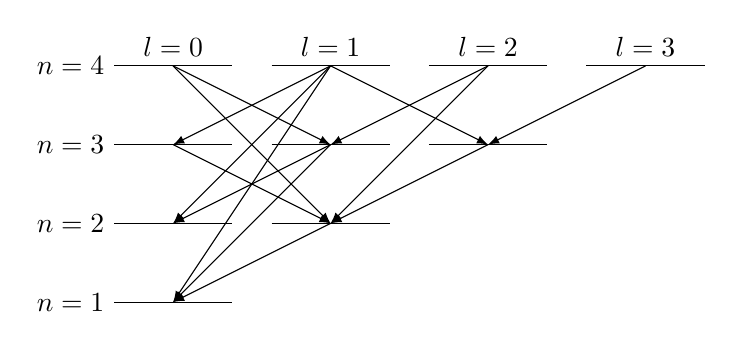
\begin{tikzpicture}
\pgfmathsetmacro{\kx}{1.5}
\pgfmathsetmacro{\ky}{1}
\pgfmathsetmacro{\ks}{0.5}
\draw[] (0,0) node[left]{$n=1$} --++ (\kx,0);
%
\draw[] (0,\ky) node[left]{$n=2$} --++ (\kx,0);
\draw[] (\kx+\ks,\ky) --++ (\kx,0);
%
\draw[] (0,2*\ky) node[left]{$n=3$} --++ (\kx,0);
\draw[] (\kx+\ks,2*\ky) --++ (\kx,0);
\draw[] (2*\kx+2*\ks,2*\ky) --++ (\kx,0);
%
\draw[] (0,3*\ky) node[left]{$n=4$} --++ (\kx,0) node[pos=0.5,above]{$l=0$};
\draw[] (\kx+\ks,3*\ky) --++ (\kx,0)node[pos=0.5,above]{$l=1$};
\draw[] (2*\kx+2*\ks,3*\ky) --++ (\kx,0)node[pos=0.5,above]{$l=2$};
\draw[] (3*\kx+3*\ks,3*\ky) --++ (\kx,0)node[pos=0.5,above]{$l=3$};
%
\draw[-latex] (\kx/2,3*\ky) --++ (\kx+\ks,-\ky);
\draw[-latex] (\kx/2,3*\ky) --++ (\kx+\ks,-2*\ky);
%
\draw[-latex] (\kx+\ks+\kx/2,3*\ky) --++ (-\kx-\ks,-\ky);
\draw[-latex] (\kx+\ks+\kx/2,3*\ky) --++ (-\kx-\ks,-2*\ky);
\draw[-latex] (\kx+\ks+\kx/2,3*\ky) --++ (-\kx-\ks,-3*\ky);
\draw[-latex] (\kx+\ks+\kx/2,3*\ky) --++ (\kx+\ks,-\ky);
%
\draw[-latex] (2*\kx+2*\ks+\kx/2,3*\ky) --++ (-\kx-\ks,-\ky);
\draw[-latex] (2*\kx+2*\ks+\kx/2,3*\ky) --++ (-\kx-\ks,-2*\ky);
%
\draw[-latex] (3*\kx+3*\ks+\kx/2,3*\ky) --++ (-\kx-\ks,-\ky);
%
\draw[-latex] (0*\kx+0*\ks+\kx/2,2*\ky) --++ (\kx+\ks,-\ky);
%
\draw[-latex] (1*\kx+1*\ks+\kx/2,2*\ky) --++ (-\kx-\ks,-\ky);
\draw[-latex] (1*\kx+1*\ks+\kx/2,2*\ky) --++ (-\kx-\ks,-2*\ky);
%
\draw[-latex] (2*\kx+2*\ks+\kx/2,2*\ky) --++ (-\kx-\ks,-1*\ky);
%
\draw[-latex] (1*\kx+1*\ks+\kx/2,1*\ky) --++ (-\kx-\ks,-1*\ky);
\end{tikzpicture}
\caption{ہائیڈروجن کی اولین چار سطحوں کی اجازتی  تنزل۔}
\label{شکل_تابع_وقت_اضطراب_اجازتی_تنزل}
\end{figure}

 
 
\ابتدا{سوال}
مساوات \num{9.74} میں دیگئی  مقلوبی  رشتہ ثابت کریں۔ اشارہ: پہلے درج ذیل دیکھائیں
\begin{align*}
	[L^2, z] = 2i\hbar(xL_y-yL_x-i\hbar z)
\end{align*}
اس کو اور \(r.L = r.(r\times p) = 0\) کو استعمال کر کے درج ذیل دیکھائیں
\begin{align*}
[L^2, [L^2, z]] = 2\hbar^2(zL^2+L^2z)	
\end{align*}
\عددی{z} سے \عددی{r} تک عمومیت دینا حقیر سا  کام ہے۔
\انتہا{سوال}
\ابتدا{سوال}
دیکھائیں کہ \(l^\prime = l = 0\) کی صورت میں \(\langle n^\prime l^\prime m^\prime \abs{r}nlm \rangle = 0\) ہوگا۔ اس سے مساوات \num{9.78} میں درپیش کمی ختم ہوگی۔
\انتہا{سوال}
\ابتدا{سوال}
ہائڈروجن کے \(n = 3, l = 0, m = 0\) حال میں ایک الیکٹران زمینی حال تک کئی برقی جفت کتب تحویل کے زریع پہنچتا ہے۔

(الف) اس تنزل کے لیئے کونسی راہیں کھلی ہیں؟ انہیں درج ذیل صورت میں پیش کریں۔
\begin{align*}
	\mid300\rangle\rightarrow \mid nlm\rangle\rightarrow \mid n^\prime l^\prime m^\prime \rangle\rightarrow\dots\rightarrow\mid100\rangle
\end{align*}
(ب) اگر آپ کے پاس ایک بوتل اس حال میں جوہروں سے بھرا ہوا ہے تب ہر راستے سے کتنا حصہ گزرے گا؟

(ج) اس حال کا عرصہ حیات کیا ہوگا؟ اشارہ: پہلی تحویل کے بعد یہ حال \(\mid300\rangle\) میں نہیں ہوگا لحاظہ اس ترتیب میں ہر  مرتبہ  صرف پہلا قدم حل کر کے متعلقہ عرصہ حیات حاصل ہوگا۔ متعدد آزاد راستوں کی صورت میں تحویلی شرح ایک دوسرے کے ساتھ جمع ہوں گی۔
\انتہا{سوال}

%======================
\حصہء{مزید سوالات برائے باب \حوالہ{باب_تابع_وقت_نظریہ_اضطراب}}
\ابتدا{سوال}
متعدد سطحی نظام کے لیئے مساوات \num{9.1} اور مساوات \num{9.2} 
\begin{align}
	H_0\psi_n = E_n\psi_n, \langle \psi_n\mid\psi_m \rangle = \delta_{nm}
\end{align}
کو عمومیت دیتے ہوئے تابع وقت نظریہ اضطراب  مرتب کریں۔ لمحہ \(t=0\) پر ہم اس اضطراب \(H^\prime(t)\) چالو کرتے ہیں۔ یوں کل ہیملٹنی درج ذیل ہوگا۔
\begin{align}
	H = H_0 + H^\prime(t)
\end{align}
(الف) مساوات \num{9.6} کی تعمیمی صورت درج ذیل ہوگی۔
\begin{align}
	\psi(t) = \sum c_n(t)\psi_ne^{-iE_nt/\hbar}
\end{align}
دیکھائیں کہ درج ذیل ہوگا
\begin{align}
	c_m = -\frac{i}{\hbar}\sum_{n} c_nH^\prime_{mn}e^{i(E_m-E_n)t/\hbar}
\end{align}
جہاں \(H^\prime_{mn}\) درج ذیل ہے
\begin{align}
	H^\prime_{mn} \equiv \langle \psi_m\abs{H^\prime}\psi_n \rangle
\end{align}
(ب) اگر نظام حال \(\psi_N\) میں آغاز کریں تب دیکھائیں کہ رتبہ اوّل نظریہ اضطراب میں درج ذیل
\begin{align}
	c_N(t)\cong1-\frac{i}{\hbar}\int_{0}^{t}H^\prime_{NN}(t^\prime)dt^\prime
\end{align}
اور درج ذیل ہوگا
\begin{align}
	c_m(t)\cong-\frac{i}{\hbar}\int_{0}^{t}H^\prime_{mN}(t^\prime)e^{i(E_m-E_N)t^\prime/\hbar}dt^\prime \quad(m\neq N)
\end{align}
(ج) فرض کریں لمحہ \(t=0\) پر چالو اور بعد میں لمحہ \عددی{t} پر منقتع کرنے کے علاوہ \(H^\prime\) مستقل ہے۔ حال \عددی{N} سے حال \(M(M\neq N)\) میں تحویل کے احتمال کو \عددی{t} کا تفاعل لکھیں۔ جواب:
\begin{align}
	4\abs{H^\prime_{MN}}^2\frac{\sin^2[(E_N-E_M)t/2\hbar]}{(E_N-E_M)^2}
\end{align}
(د) فرض کریں \(H^\prime\) وقت کا سائن نما تفاعل \(H^\prime=V\cos(\omega t)\) ہے۔ عمومی مفروضے فرض کرتے ہوئے دیکھائیں کہ صرف توانائی \(E_M = E_N\pm\hbar\omega\) کے حالات میں تحویل ہوسکتی ہے اور انکا احتمال درج ذیل ہے۔
\begin{align}
	P_{N\rightarrow M} = \abs{V_{MN}}^2\frac{\sin^2[(E_N-E_M\pm\hbar\omega)t/2\hbar]}{(E_N-E_M\pm\hbar\omega)^2}
\end{align}
(و) فرض کریں ایک متعدد سطحی نظام پر غیر اتساکی برقناطیسی روشنی ڈالی جاتی ہے۔ حصہ 9.2.3 کو دیکھتے ہوئے دیکھائیں کہ دو سطحی نظام کے لیئے تحرقی اخراج کی تحویلی شرح وہی کلیہ مساوات \num{9.47} دیگا۔
\انتہا{سوال}
\ابتدا{سوال}
عددی سر \(c_m(t)\) کو رتبہ اوّل تک سوال \num{9.15} (ج) اور (د) کے لیئے تلاش کریں۔ معمولزنی شرط 
\begin{align}
	\sum_{m}\abs{c_m(t)}^2 = 1
\end{align}
کی تصدیق کر کے تزاد اگر موجود ہو پر تبصرہ کریں۔ فرض کریں آپ ابتدائی حال \(\psi_N\) میں رہنے کا احتمال جاننا چاہتے ہیں۔ کیا \(\abs{c_N(t)}^2\) یا \(1-\sum_{m\neq N}\abs{c_m(t)}^2\) کا استعمال بہتر ثابت ہوگا؟
\انتہا{سوال}
\ابتدا{سوال}
ایک لامتناہی چکور کنواں کہ \عددی{N}ویں حال میں وقت \(t=0\) پر ایک ذرہ آغاز کرتا ہے۔ وقتی طور پر کنواں کی تہ بلند ہو کر واپس اپنی جگہ نیچے بیٹھتی ہے جس کے تحت کنواں کے اندر مخفیہ یکساں ضرور لیکن تابع وقت ہوگی \(V_0(t)\) جہاں \(V_0(0) = V_0(T) = 0\) ہوگا۔

(الف) مساوات \num{9.82} استعمال کرتے ہوئے \(c_m(t)\) کی ٹھیک ٹھیک قیمت دریافت کریں اور دیکھائیں کہ تفاعل موج کی حیط زاویائی دور تبدیل ہوگا لیکن تحویل نہیں ہوگی۔ تفاعل \(V_0(t)\) کی صورت میں تبدیلی حیط، تبدیلی زاویائی دور \(\psi(T)\) تلاش کریں۔

(ب) اسی مسئلہ کو رتبہ اوّل نظریہ اضطراب سے حل کر کے دونوں نتائج کا موازنہ کریں۔

تبصرہ: ہر  اُس صورت میں جب مخفیہ کے ساتھ اضطراب \عددی{x} میں مستقل نا کے \عددی{t} میں جمع کرتا ہو یہی نتیجہ حاصل ہوگا۔ یہ صرف لامتناہی چکور کنواں کی خاصیت نہیں ہے۔ سوال \num{1.8} کے ساتھ موازنہ کریں۔
\انتہا{سوال}

%============================

\ابتدا{سوال}
ایک بُعدی لامتناہی چکور کنواں کی زمینی حال میں کمیت \عددی{m} کا ایک ذرہ ابتدائی طور پر پایا جاتا ہے۔ لمحہ \(t=0\) پر ایک اینٹ اس کنواں میں گرائی جاتی ہے جس سے مخفیہ درج ذیل ہو جاتا ہے جہاں \(V_0<<E_1\) ہے۔
\begin{align*}
	V(x)=
	\begin{cases}
		V_0 & 0\leq x\leq a/2 \text{\RL{جب}} \\
		0 & a/2<x\leq a \text{\RL{جب}} \\
		\infty & \text{\RL{دیگرصورت}}
	\end{cases}
\end{align*}
کچھ وقت \عددی{T} کے بعد اینٹ ہٹائی جاتی ہے اور ذرہ کی توانائی ناپی جاتی ہے۔ رتبہ اوّل نظریہ اضطراب میں نتیجہ \عددی{E_2} ہونے کا احتمال کیا ہوگا؟
\انتہا{سوال}
\ابتدا{سوال}
ہم تحرقی اخراج، تحرقی انجزاب اور خود با خود اخراج دیکھ چکے ہیں۔ خود با خود انجزاب کیوں نہیں پایا جاتا ہے؟
\انتہا{سوال}
\ابتدا{سوال}
مقناطیسی گمک ساکن مقناطیسی میدان \(B_0\ak\) میں \(1/2\) چکر کا ایک ذرہ جس کی مسکن مقناطیسی نسبت \(\gamma\) ہو لارمر تعدد \(\omega_0 = \gamma B_0\) مثال \num{4.3} سے استقبالی حرکت کرتا ہے۔ اب ہم ایک کمزور عارضی ریڈیائی تعدد میدان \(B_{rf}[\cos(\omega t)\ai-\sin(\omega t)\aj]\) چالو کرتے ہیں جس سے کل میدان درج ذیل ہو جاتا ہے۔
\begin{align}
	B = B_{rf}\cos(\omega t)\ai - B_{rf}\sin(\omega t)\aj + B_0\ak
\end{align} 
(الف) اس نظام کے لیئے \(2\times2\) ہیملٹی قالب مساوات \num{4.158} تیار کریں۔

(ب) وقت \عددی{t} پر \(\chi(t) = \begin{pmatrix}a(t) \\b(t)\end{pmatrix}\) چکر حال ہونے کی صورت میں درج ذیل دیکھائیں۔
\begin{align}
	\dot{a} = \frac{i}{2}\big(\Omega e^{i\omega t}b+\omega_0 a\big):\quad\dot{b} = \frac{i}{2}\big(\Omega e^{i\omega t}a-\omega_0 b\big)
\end{align}
جہاں \(\Omega\equiv\gamma B_{rf}\) کا تعلق ریڈیائی تعدد میدان کی زور کے ساتھ پایا جاتا ہے۔

(ج) ابتدائی قیمتیں \عددی{a_0} اور \عددی{b_0} کی صورت میں \عددی{a(t)} اور \عددی{b(t)} کا عمومی حل تلاش کریں۔ جواب: 
\begin{align*}
	a(t) &= \bigg\{a_0\cos(\omega^\prime t/2)+\frac{i}{\omega^\prime}[a_0(\omega_0-\omega)+b_0\Omega]\sin(\omega^\prime t/2)\bigg\}e^{i\omega t/2} \\
	b(t) &= \bigg\{b_0\cos(\omega^\prime t/2)+\frac{i}{\omega^\prime}[b_0(\omega-\omega_0)+a_0\Omega]\sin(\omega^\prime t/2)\bigg\}e^{-i\omega t/2}
\end{align*}
جہاں درج ذیل ہوگا
\begin{align}
	\omega^\prime\equiv\sqrt{(\omega-\omega_0)^2+\Omega^2}
\end{align}
(د) ہواں میدان چکر حال یعنی \(a_0 = 1, b_0 = 0\) سے ایک ذرہ آغاز کرتا ہے۔ مخالف میدان چکر میں تحویل کی احتمال کو بطور وقت کا تفاعل تلش کریں۔

جواب: \(P(t) = \{\Omega^2/[(\omega-\omega_0)^2+\Omega^2]\}\sin^2(\omega^\prime t/2)\)

(و) منحنی گمک
\begin{align}
	P(\omega) = \frac{\Omega^2}{(\omega-\omega_0)^2+\Omega^2}
\end{align}
کو غیر متغیر \(\omega_0\) اور \(\Omega\) کیصورت میں متحرق تعدد \(\omega\) کی تفاعل کے طور پر ترسیم کریں۔ آپ دیکھیں گے کہ \(\omega = \omega_0\) پر اس کی زیادہ سے زیادہ قیمت پائی جاتی ہے۔ زیادہ سے زیادہ قیمت کی نصف پر پوری چوڑائی \(\Delta\omega\) تلاش کریں۔

(ھ) چونکہ \(\omega_0 = \gamma B_0\) ہے لحاظہ ہم تجرباتی طور گمک کا مشاہدہ کر کے ذرہ کی مقناطیسی جفت کتب معیارِ اثر تعین کر سکتے ہیں۔ ایک مرکزی مقناطیسی گمک تجربہ میں فوٹان کا \عددی{g} جزو ضربی ایک ٹیسلا کے ساکن میدان اور ایک مائکرو ٹیسلا حیطہ کے ریڈیائی تعدد میدان کی مدد سے ناپا جاتا ہے۔ تعدد گمک کیا ہوگا؟ پروٹان کی مقناطیسی معیارِ اثر کے لیئے حصۃ \num{6.5} دیکھیں۔ منحنی گمک کی چوڑائی تلاش کریں۔ اپنا جواب \(\si{\hertz}\) میں دیں۔
\انتہا{سوال}
\ابتدا{سوال}
میں نے مساوات \num{9.31} میں فرض کیا تھا کہ جوہر روشنی کی طولِ موج کے لحاظ سے اتنا چھوٹا ہے کہ میدان کی فضائی تغیر کو نظر انداز کیا جا سکتا ہے۔ حقیقی برقی میدان درج ذیل ہوگا
\begin{align}
	E(r,t) = E_0\cos(k.r-\omega t)
\end{align}
اگر جوہر کا مرکز مبدا پر ہو تب متعلقہ حجم پر \(k.r<<1\) \((\abs{k} = 2\pi/\lambda, \text{\RL{لحاظہ}}k.r\sim r/\lambda<<1)\) ہوگا جس کی بنا ہم اس جزو کو نظرانداز کر سکتے تھے۔ فرض کریں ہم رتبہ اوّل درستگی۔
\begin{align}
	E(r,t) = E_0[\cos(\omega t)+(k.r)\sin(\omega t)]
\end{align}
استعمال کریں۔ اس کا پہلا جزو وہ اجازتی برقی جفت کتب تحویلات پیدا کرتا ہے جن پر متن میں بات کی چکی ہے۔ دوسرا جزو وہ تحویلات پیدا کرتا ہے جنہیں ممنوعہ مقناطیسی جفت کتب اور برقی چو کتب تحویل کہتے ہیں \(k.r\) کی اس سے زیادہ بڑی طاقتیں مزید زیادہ ممنوعہ تحویلات پیدا کرتی ہے جو زیادہ بلند متعدد کتبی معیارِ اثر کے ساتھ وابستہ ہوں گے۔

(الف) ممنوعہ تحویلات کی خود با خود اخراجی شرح حاصل کریں اس کی تکتیب اور حرکت کے رخ پر اوسط قیمت تلاش کرنے کی ضرورت نہیں ہے اگر چہ مکمل جواب کے لیئے ایسا کرنا ضروری ہوگا۔ جواب:
\begin{align}
	R_{b\rightarrow a} = \frac{q^2\omega^5}{\pi\epsilon_0\hbar c^5}|\langle a|(\kvecsub{a}{n}.r)(\ak.r)|b \rangle|^2
\end{align}
(ب) دیکھائیں کہ ایک بُعدی مرتعش کے لیئے ممنوعہ تحویلات سطح \عددی{n} سے سطح \(n-2\) میں ہوگی اور تحویلی شرح جس کی اوسط قیمت \(\kvecsub{a}{n}\) اور \(\ak\) پر حاصل کی گئی ہو درج ذیل ہوگا۔
\begin{align}
	R = \frac{\hbar q^2\omega^3n(n-1)}{15\pi\epsilon_0m^2c^5}
\end{align}
تبصرہ: یہاں \(\omega\) سے مراد فوٹان کا تعدد ہے نا کہ مرتعش کا تعدد۔ اجازتی شرح کے لحاظ سے ممنوعہ شرح کا نصبط تلاش کریں۔ ان اصطلاح پر تبصرہ کریں۔

(ج) دیکھائیں کہ ہائڈروجن میں ممنوعہ تحویل بھی \(2S\rightarrow 1S\) کی اجازت نہیں دیتا۔ درحقیقت یہ تمام بلند متعدد کتب کے لیئے بھی درست ہوگا غالب تنزل دو فوٹان اخراج کی بنا ہوگا جس کا عرصہ حیات تقریباً ایک  سیکنڈ کا دسواں حصہ ہوگا۔
\انتہا{سوال}
\ابتدا{سوال}
دیکھائیں کہ \عددی{n,l} سے \(n^\prime, l^\prime\) میں تحویل کے لیئے ہائڈروجن کا خود با خود اخراجی شرح مساوات \num{9.56} درج ذیل ہوگا۔
\begin{align}
	\frac{e^2\omega^3I^2}{3\pi\epsilon_0\hbar c^3}\times
	\begin{cases}
		\frac{l+1}{2l+1}, & l^\prime = l+1 \text{\RL{جب}} \\
		\frac{l}{2l-1}, & l^\prime = l-1 \text{\RL{جب}}
	\end{cases}
\end{align}
جہاں \عددی{I} درج ذیل ہے۔
\begin{align}
	I\equiv\int_{0}^{\infty} r^3R_{nl}(r)R_{n^\prime l^\prime}(r)dr
\end{align}
جوہر \عددی{m} کی کسی مخصوص قیمت سے آغاز کر کے انتخابی قواعد \(m^\prime = m+1, m, \text{\RL{یا}} m-1\) کے تحت \(m^\prime\) حالات میں سے کسی ایک میں پہنچتا ہے۔ دیہان رہے کہ جواب \عددی{m} پر منحصر نہیں ہے۔ اشارہ: پہلے \(l^\prime = l+1\) صورت کے لیئے \(\mid nlm\rangle\) اور \(\mid n^\prime l^\prime m^\prime \rangle\) کے بیچ \عددی{x, y} اور \عددی{z} کے تمام غیر صفر قالبی ارکان معلوم کریں۔ ان سے درج ذیل مقدار تعین کریں
\begin{align*}
	|\langle n^\prime, l+1,m+1\abs{r}nlm \rangle|^2 + |\langle n^\prime, l+1, m\abs{r}nlm \rangle|^2+|\langle n^\prime, l+1, m-1\abs{r}nlm\rangle|^2
\end{align*}
یہی کچھ \(l^\prime = l-1\) کے لیئے بھی کریں۔
\انتہا{سوال}

%===================
